

\documentclass[a4paper,10pt]{book}
\usepackage{amsmath}
\usepackage{amscd}
\usepackage{amssymb}
\usepackage{graphicx}
\usepackage{subfigure}  % per le sottofigure
\usepackage{makeidx}
\usepackage[square,longnamesfirst]{natbib}     % bibliografia
\usepackage{empheq}
\usepackage{tikz}       % per i grafici/diagrammi scritti
\usepackage{hyperref}

\usepackage[utf8x]{inputenc}
\usepackage[italian]{babel}

\definecolor{MyGray}{rgb}{0.96,0.97,0.98}
\makeatletter\newenvironment{graybox}{%
   \begin{lrbox}{\@tempboxa}\begin{minipage}{\columnwidth}}{\end{minipage}\end{lrbox}%
   \colorbox{MyGray}{\usebox{\@tempboxa}}
}\makeatother

\newenvironment{esempio}
{\subsubsection{Esempio}}
{} 

\newenvironment{dimostrazione}
{\subsubsection{Dimostrazione}}
{}



\makeindex

\title{Identificazione dei modelli ed analisi dei dati}
\author{Federico Vaga}
\date{Gennaio 2011}
\begin{document}
\maketitle  % stampa titolo e autore

% stampa la licenza CC BY-NC-SA_2.5_IT
% occorre che i documento originale usi il pacchetto hyperref

\begin{center}\textbf{{\large Licenza - License}}\end{center}

\begin{figure}[hcbp]  
  \centering
  
\includegraphics{../licenza/CreativeCommons/BY-NC-SA_2.5_IT/cc.png}
\end{figure}

\begin{center}\textbf{Italiano}\end{center}
“Questo lavoro è licenziato sotto licenza Creative Commons - Non commerciale - Condividi allo stesso modo 2.5 Italia (CC BY-NC-SA 2.5). Per vedere una copia di questa licenza visita il sito \url{http://creativecommons.org/licenses/by-nc-sa/2.5/it/}; oppure invia una lettera a Creative Commons, 171 2nd Street, Suite 300, San Francisco, California, 94105, USA.”\newline
\begin{center}\textbf{English}\end{center}
“This work is licensed under the Creative Commons Attribuzione - Non commerciale - Condividi allo stesso modo 2.5 Italia (CC BY-NC-SA 2.5) License. To view a copy of this license, visit \url{http://creativecommons.org/licenses/by-nc-sa/2.5/it/}; or, (b) send a letter to Creative Commons, 171 2nd Street, Suite 300, San Francisco, California, 94105, USA.” \newline


\begin{center}
\textbf{Note}
\end{center}
Questo lavoro è basato principalmente su una revisione degli appunti \cite{unpub:imadls} raccolti durante il corso \href{http://www-3.unipv.it/ingegneria/didattica/schedacorso1011.php?cod=064050&spec=0}{identificazione dei modelli ed analisi dei dati LS} tenuto dal professor Giuseppe De Nicolao presso l'Università degli studi di Pavia. Il lavoro è inoltre integrato dalla lettura del libro \textit{Identificazione parametrica} \cite{book:identificazioneparametrica}

\tableofcontents % stampa l'indice

\part{Teoria della stima}
% TEORIA DELLA STIMA
\chapter{Teoria della stima}
  % Introduzione
  \section{Introduzione}

Molto spesso, durante l'analisi dei dati, non sono note le densità di probabilità - ddp - ma sono disponibili solo dei dati sperimentali, quindi vorremmo poter estrarre informazioni dai dati per procedere ad un'analisi statistica; il processo di estrazione di queste informazioni è il processo di stima. Il processo di stima di un'informazione (parametro) si basa sull'uso dello stimatore \index{Stimatore}, ovvero, una funzione deterministica che è in grado di calcolare un parametro in funzione dei dati disponibili. In letteratura esistono molti stimatori per particolari parametri, ma in generale come si crea uno stimatore?

\begin{figure}[htbp]
  \centering
  \[
    \begin{CD}
      \framebox{$\theta^0$} @>>> \framebox{$f_X^{\theta^0}(x)$} @>X>> \framebox{$g(X)$} @>>> \framebox{$\hat{\theta}$}
    \end{CD}
  \]
  \caption{Diagramma di stima\label{fig:diagrammastima}}
\end{figure}



$\theta^0$  è un vettore di parametri \index{Parametri} che vengono usati per generare l'esperimento. Alcuni o tutti questi parametri sono ignoti e sarà nostro compito stimarne il valore. \newline

$f_X^{\theta^0}(x)$ è una funzione di densità congiunta che dai parametri genera i dati sperimentali \newline

$g(X)$ è la funzione stimatore; a partire dai dati sperimentali fornisce un valore di stima per i parametri $\theta^0$ \newline

$\hat{\theta}$ è il vettore che stima i parametri

Dato che il risultato dello stimatore è una variabile casuale - V.C. - non è detto che la sua stima sia esatta; quello che si cerca di fare è far sì che il valore di stima sia il più possibile vicino al valore esatto con un errore, possibilmente, piccolo.

\begin{esempio}

Stimare la media $m$ e la deviazione standard $\sigma$ di una V.C. gaussiana

  \[ \theta^0=\begin{bmatrix}\theta_1^0 \\ \theta_2^0  \end{bmatrix}=\begin{bmatrix} m \\ \sigma \end{bmatrix} \]

Noi sappiamo che i dati sperimentali sono generati a partire da dei particolari parametri:
% ci avevo messo qualcosa ma nn ricordo cosa
in questo caso da media e deviazione standard. Questi sono i veri parametri dell'esperimento ma che sono a noi ignoti, in quanto, disponiamo solo dei dati sperimentali. Sappiamo però che le V.C. che fanno riferimento ai singoli dati sono gaussiane e quindi hanno una ddp a noi nota:

    \[ f_{X_i}^{\theta^0}(x_i)= \frac{1}{\sqrt{2\pi \theta_2^0} }e^{- \frac{1}{2} \left( \frac{(x_i-\theta_1^o)}{\theta_2^0} \right) ^2}  \]

La nostra ddp congiunta dell'esperimento è data dalla produttoria di tutte le ddp dei dati, quindi, supponendo di avere $N$ dati avremo:

    \[ f_X^{\theta^0}(x)=\prod_{i=1}^{N} f_{X_i}^{\theta^0}(x_i)  = \frac{1}{\sqrt{(2\pi \theta_2^0)^N} }e^{- \frac{1}{2}  \sum_{i=1}^{N}{ \left( \frac{(x_i-\theta_1^o)}{\theta_2^0} \right) ^2}  } \]

usando ora una funzione stimatrice, ad esempio la media campionaria per la media, possiamo scrivere:

  \[
    \hat{\theta} = \begin{bmatrix} \hat{\theta}_1 \\ \hat{\theta}_2 \end{bmatrix} =  \begin{bmatrix} g_1(X) \\ g_2(X) \end{bmatrix} , \quad g_1(X)=\frac{1}{N}\sum _{i=1} ^{N} {x_i}
  \]
\end{esempio}

   % Proprietà degli stimatori
  \section{Proprietà degli stimatori}
Gli stimatori possono godere di alcune proprietà. Le proprietà di maggiore interesse sono:
  \begin{itemize}
     \item polarizzazione
     \item consistenza
     \item asintottica normalità
   \end{itemize}
% ######################################################################## Polarizzazione
\subsection{Polarizzazione}
La polarizzazione \index{Polarizzazione} indica lo scostamento della stima $\hat{\theta}$ rispetto al valore esatto $\theta^0$: se uno stimatore è non polarizzato, non c'è alcun scostamento rispetto al valore esatto e la sua ddp è centrata su di esso quindi $E[\hat{\theta}]=\theta^0$; altrimenti è polarizzato e scriviamo $E[\hat{\theta}]\ne \theta^0$. In figura \ref{fig:espolarizzazione} lo stimatore $f_{\hat{\theta}_1}$ è non polarizzato, mentre lo stimatore $f_{\hat{\theta}_2}$ è polarizzato. 

  \begin{figure}[htbp]
    \centering
    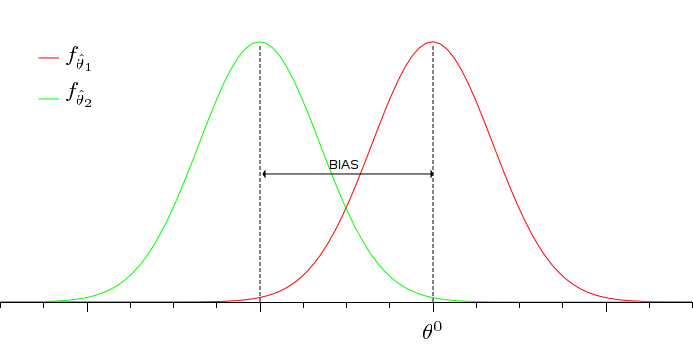
\includegraphics[scale=0.6]{img/polarizzazione.png}
    \caption{esempio di polarizzazione\label{fig:espolarizzazione}}
  \end{figure}

In uno stimatore polarizzato, la differenza fra il valore atteso dello stimatore ed il valore vero è definito BIAS:

    \[ BIAS=E[\hat{\theta}]-\theta^0 \]

In linea di massima è preferibile uno stimatore non polarizzato, ma esistono alcuni casi in cui può essere conveniente usare uno stimatore polarizzato. 


% ######################################################################## Consistenza
\subsection{Consistenza}
La consistenza \index{Consistenza} è una proprietà molto desiderabile in quanto essa definisce la capacità di uno stimatore di concentrare i propri valori al crescere del numero di campioni considerati in un esperimento; se uno stimatore è consistente, per grandi campioni, avremo una varianza piccola attorno ad un valore e quindi una migliore stima, inoltre, se lo stimatore è non polarizzato all'aumentare dei campioni questi tendono a concentrarsi attorno al valore esatto \footnote{Idealmente per infiniti campioni diventa una delta di Dirac su valore esatto} come rappresentato in figura \ref{fig:esconsistenza}

\begin{figure}[htbp]
  \centering
  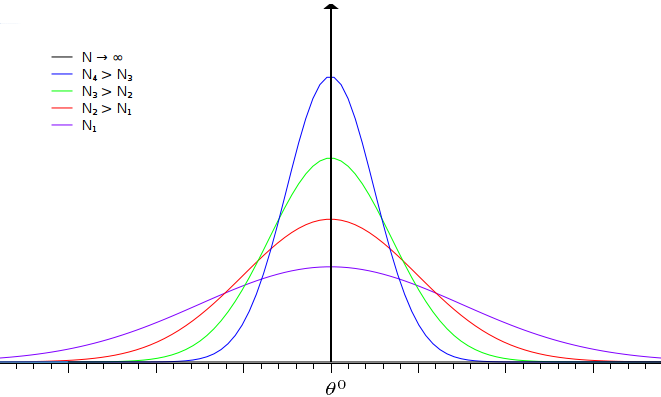
\includegraphics[scale=0.5]{img/G2D.png}
  \caption{esempio consistenza\label{fig:esconsistenza}}
\end{figure}

% ########################################################################
\subsection{Asintottica normalità}
L'asintotica normalità \index{Asintottica normalità}, definisce la capacità di uno stimatore di tendere ad una distribuzione gaussiana all'aumentare dei campioni acquisiti.
% ######################################################################## disuguaglianza CR
\subsection{Disuguaglianza di Cramer-Rao}
Con la disuguaglianza di Cramer-Rao \index{Limite Cramer Rao} - CR - si definisce un limite inferiore per la varianza oltre il quale la stima non può migliorare:

    \[ Var[\hat{\theta}]\geq - \left( E\left[\frac{\partial^2}{\partial\theta^2} ln f_X^\theta(X)\mid_{\theta=\theta^0}\right] \right)^{-1} = S^{-1} \]

Per uno stimatore non polarizzato la varianza è sinonimo di precisione, quinidi, una varianza minore significa maggiore precisione e quindi è da preferire. Da questa disuguaglianza ne consegue che non è possibile ottenere uno stimatore con una varianza inferiore al limite di CR. Il limite CR esiste perché, dopotutto, dai dati sperimentali non si può ricavare più di tanto e un margine di incertezza rimane sempre: il risultato ideale a varianza nulla è impossibile da ricavare puntualmente.\newline
La quantità utilizzata per definire il limite CR è detta \textit{quantità di informazione di Fisher} \index{Quantità di informazione di Fisher}:

    \[ S:= -  E\left[\frac{\partial^2}{\partial \theta^2} ln f_X^\theta(X)\mid_{\theta=\theta^0}\right] \]

Per un caso vettoriale, avremo una matrice di informazione:

\begin{gather*}
  S= \{ S_{ij}\}  \\
  S_{ij}:= -  E\left[\frac{\partial^2}{\partial \theta_i\partial \theta_j} ln f_X^\theta(X)\mid_{\theta=\theta^0}\right]
\end{gather*}

Il limite CR è definito solo per stimatori non polarizzati, ma esiste una legge analoga anche per il caso di stimatori polarizzati.
% ######################################################################## Conclusioni
\subsection{Conclusioni}
Come prima osservazione, uno stimatore inconsistente deve destare sospetti perché non riusciremmo a stimare precisamente un parametro dato che all'aumentare dei campioni non ci vengono fornite nuove informazioni, mentre è desiderabile che avvenga il contrario fino a tendere ad una stima precisa.\newline
Generalmente, come già accennato, è preferibile uno stimatore non polarizzato, ma potrebbe capitare che sia più utile uno polarizzato; ad esempio potrebbe essere preferibile uno stimatore poco polarizzato ma che ha una varianza molto piccola rispetto ad uno stimatore non polarizzato ma con un'ampia varianza.

\begin{figure}[htbp]
  \centering
  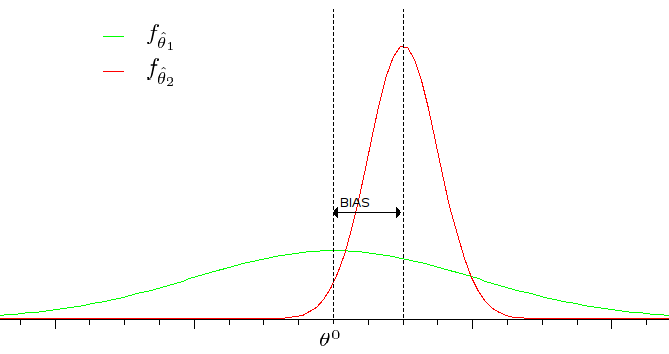
\includegraphics[scale=0.5]{img/npfm.png}
  \caption{Confronto fra stimatore polarizzato consistente e uno non polarizzato e non consistente\label{fig:confrontopolarizzazioneconsistenza}}
\end{figure}

Come si vede in figura \ref{fig:confrontopolarizzazioneconsistenza}, nel caso dello stimatore polarizzato $f_{\hat{\theta}_2}$, i valori che ci vengo forniti sono in un intorno piccolo vicino al valore esatto, quindi anche se sappiamo di sbagliare la stima, sappiamo anche che stiamo sbagliando di poco rispetto allo stimatore non polarizzato $f_{\hat{\theta}_1}$ che invece ha un ampio margine di errore. Infatti, lo stimatore polarizzato è più consistente rispetto al non polarizzato e come visto in precedenza, la consistenza è una proprietà molto desiderabile. L'ideale sarebbe spostare lo stimatore polarizzato di modo da centrarlo e quindi renderlo non polarizzato.\newline
Abbiamo appena dimostrato che uno stimatore polarizzato potrebbe essere preferibile, ma come possiamo valutare analiticamente la sua precisione? Quello che possiamo fare è valutare l'errore quadratico medio (mean square error):

    \[ E[(\hat{\theta}-\theta^0)^2] \approxeq 0\]

Il motivo per cui si valuta l'errore quadratico e non l'errore, è che valutando l'errore è facile ottenere $E[\hat{\theta}-\theta^0]=0$ mediante compensazione fra errori positivi ed errori negativi, mentre con l'errore quadratico ciò non capita.\newline
%FIXME
    \begin{center}
    \textbf{[FIXME i famosi conti che non capisco]}
    \end{center}
Dalla formula appena illustrata, possiamo concludere che lo stimatore polarizzato è accettabile se si guadagna abbastanza in varianza o, viceversa, preferire la non polarizzazione perdendo in varianza. Uno stimatore non polarizzato $\hat{\theta}^m$ si dice a minima varianza \index{minima varianza} se:

    \[ Var[\hat{\theta}^m]\leq Var[\hat{\theta}],\quad\forall \hat{\theta} \]

Questo significa che lo stimatore non polarizzato è a minima varianza se la sua varianza è minore, o uguale, alla varianza di un qualisasi altro stimatore non polarizzato. Se uno stimatore ha la varianza che raggiunge il limite CR \index{Limite Cramer Rao} allora è sicuramente a varianza minima; non è detto che ogni stimatore possa raggiungere il limite CR, ma ciò non vieta l'esistenza della minima varianza.

  % Stima dei momenti di una variabile casuale: momenti campionari
  \section{Stima dei momenti di una variabile casuale: momenti campionari}
% ######################################################################## Dai momenti ai momenti campionari
\subsection{Dai momenti ai momenti campionari}

Nel nostro classico problema di stima abbiamo a che fare con un esperimento casuale che fornisce $N$ valori $X_i$,  V.C. indipendenti ed identicamente distribuite\footnote{significa che hanno tutte la stessa densità di probabilità -ddp-} - iid - con $f_{X_i}(x_i)$ nota. Dato che le V.C. sono iid possiamo scrivere: 

    \[ f_X(x)=\prod_{i=1}^{N}{f_{X_i}(x_i)} \]

inoltre, sappiamo: 

  \begin{align*}
      E[X_i]&=m, \forall i \\
    Var[X_i]&=\sigma^2, \forall i
  \end{align*}
  
Da queste considerazioni, quello che vogliamo ottenere è una stima dei momenti di $X_i$. 
Nel dominio continuo, i momenti sono valori esatti che dipendono dalla ddp e possiamo scriverli come: 

  \begin{align*}
      m_k&=\int_{-\infty }^{\infty} {x^k \cdot f(x) \cdot dx} \quad &\text{momento di ordine k}\\
    \mu_k&=\int_{-\infty }^{\infty} {(x-m_1)^k \cdot f(x) \cdot dx} \quad &\text{momento centrale di ordine k}
  \end{align*}
  
Dato che non abbiamo a disposizione la ddp, non possiamo calcolare i momenti in questo modo, ma possiamo affidarci ai momenti campionari che essendo stimatori non forniscono i valori esatti, ma una V.C. dipendente dai dati\footnote{ovvero da altre V.C.}:
 
  \begin{align*}
    M_k&=\frac{1}{N}\sum_{i=1}^{N} {X_i^k} &\text{momento campionario di ordine k}\\
    S_k&=\frac{1}{N}\sum_{i=1}^{N} {(X_i-M_1)^k} &\text{momento campionario centrale di ordine k}
  \end{align*}
  
Da notare che i due tipi di momenti sono molto diversi, infatti, il momento campionario fa riferimento solo ad un particolare esperimento, per cui la sua ripetizione potrebbe far cambiare il valore del momento campionario, invece, il momento è un valore assoluto che dipende solo dalla ddp dell'esperimento, e quindi alla ripetizione dell'esperimento il momento non cambia.
% ######################################################################## Proprietà dei momenti campionari
\subsection{Proprietà dei momenti campionari}
\subsubsection{Media campionaria - momento campionario di ordine 1}%###############
Il momento campionario di ordine 1, ovvero la media campionaria \index{Media campionaria}, è uno stimatore non polarizzato:

    \[ M_1=\frac{1}{N} \sum_{i=1}^{N} X_i \]

Il valore atteso per la media campionaria è la media, infatti:

    \[ E[M_1]=E\left[\frac{1}{N}\sum_{i=1}^{N}{x_i}\right]=\frac{1}{N}E\left[\sum_{i=1}^{N}{x_i}\right]=\frac{1}{N}\sum_{i=1}^{N}{E[x_i]}=\frac{1}{N}Nm=m \]

La media campionaria è anche uno stimatore consistente, infatti la sua varianza diminuisce all'aumentare dei campioni, il che significa che i suoi valori si stanno concentrando in un particolare punto:

    \[ Var[M_1]=Var\left[\frac{1}{N}\sum_{i=1}^{N}{x_i}\right]=\frac{1}{N^2}\sum_{i=1}^{N}{Var[x_i]}=\frac{1}{N^2}N\sigma^2=\frac{\sigma^2}{N} \]

La media campionaria è anche asintotticamente normale. Sappiamo che se $f_{X_i}$ è una gaussiana, allora anche $M_1$ sarà gaussiana; mentre, se $f_{X_i}$ non è gaussiana $M_1$, per il teorema del limite centrale, tende alla gaussianità per $N\rightarrow\infty$, ovvero al crescere dei dati raccolti.\newline

%FIXME riguardarsi il significato
Infine, osserviamo che, essendo:

  \begin{gather*}
    Z:=\frac{M_1-E[M_1]}{\sqrt{Var[M_1]}}=\frac{M_1-m}{\frac{\sigma}{\sqrt{N}}} \Rightarrow M_1=m+\frac{\sigma}{\sqrt{N}}Z = m+e
    \lim_{N \rightarrow \infty}{Z}=0 
  \end{gather*}
  
possiamo concludere che:

    \[ \lim_{N \rightarrow \infty} M_1= m \]

\subsubsection{Valore quadratico medio - momento di ordine 2}%###############
Il momento campionario di ordine 2, ovvero il valore quadratico medio \index{Valore quadratico medio}, è uno stimatore non polarizzato:

    \[ M_2 = \frac{1}{N} \sum_{i=1}^{N}{x_i^2} \]

il suo valore atteso, risulta infatti:

    \[ E[M_2]=\frac{1}{N} \sum_{i=1}^{N} {E[x_i^2]}=\frac{1}{N} N m_2=m_2 \]
    
Il valore quadratico medio è anche uno stimatore consistente, infatti la sua varianza diminuisce all'aumentare dei campioni, il che significa che i suoi valori si stanno concentrando in un punto particolare:
  %FIXME Var[x^2]= ???
  \[ Var[M_2]=Var[\frac{1}{N} \sum_{i=1}^{N}{x_i^2}]=\frac{1}{N^2}\sum_{i=1}^{N}{Var[x_i^2]}=\frac{1}{N^2}NVar[x^2]=\frac{Var[x^2]}{N} \]

%FIXME Non mi è chiarissimo
Nel caso in cui le $X_i$ fossero gaussiane con $E[X_i]=0$, allora $\chi_N^2=N \frac{M_2}{\sigma^2}$

\subsubsection{Varianza campionaria - momento campionario centrale di ordine 2} %###############
Il momento campionario centrale di ordine 2, ovvero la varianza campionaria\index{Varianza campionaria}, possiede due possibilità di calcolo. La prima ha come ipotesi la conoscenza della media dell'esperimento e quindi:

    \[ S_m^2:=\frac{1}{N} \sum_{i=1}^{N}{(x_i-m)^2} \]
    
Lo stimatore così calcolato è non polarizzato, infatti:

    \[E[S_m^2]=\frac{1}{N} \sum_{i=1}^{N}{E[(x_i-m)^2]}=\frac{1}{N} \sum_{i=1}^{N}{Var[x_i]}=\frac{1}{N} N \sigma^2=\sigma^2 \]

La seconda possibilità, la più frequente, si ha quando non si conosce la media dell'esperimento e quindi si fa uso della sua stima $M_1$:

    \[ S^2:=S_2:=\frac{1}{N} \sum_{i=1}^{N}{(x_i-M_1)^2} \]

lo stimatore così ottenuto è polarizzato, infatti\footnote{$S^2=M_2-M_1^2$}\footnote{$\sigma^2=E[X^2]-m_1^2=m_2-m_1^2$}:

    \[ 
      \begin{split}
        E[S^2] &=E[M_2]-E[M_1^2]=m_2-\left( Var[M_1]+E[M_1]^2 \right) =\\ 
        &=m_2 -\frac{\sigma^2}{N}-m_1^2=(m_2-m_1^2)-\frac{\sigma^2}{N}=\sigma^2-\frac{\sigma^2}{N}=\frac{N-1}{N}\sigma^2
      \end{split} 
    \]

Dato che capita spesso di non avere a disposizione la media, si è costretti ad usare $S^2$ anche se sappiamo essere polarizzato. Quello che possiamo fare per porre rimedio alla polarizzazione è correggere questo stimatore ed usare quindi la varianza campionaria corretta \index{Varianza campionaria corretta} che non è polarizzata:
  
  \begin{align*}
      S_c^2:&=\frac{N}{N-1}S^2=\frac{N}{N-1}\frac{1}{N}\sum_{i=1}^{N}{(x_i-M_1)^2}=\frac{1}{N-1}\sum_{i=1}^{N}{(x_i-M_1)^2} \\
    E[S_c^2]&=E[\frac{N}{N-1}S^2]=\frac{N}{N-1}E[S^2]=\frac{N}{N-1}\frac{N-1}{N}\sigma^2=\sigma^2
  \end{align*}
  
Da notare però che l'operazione non è "indolore", infatti, l'aver voluto la non polarizzazione ha aumentato la varianza dello stimatore:

    \[ Var[S_c^2]=Var[\frac{N}{N-1}S^2]=\left(\frac{N}{N-1}\right)^2Var[S^2] \]

è evidente infatti che:

    \[ \frac{N}{N-1}>1 \]

e quindi la varianza cresce.

\paragraph{Teorema di Fisher} \index{Teorema di Fischer} Se $X_i$ sono V.C. gaussiane iid, allora $S^2$ è una $\chi_{N-1}^2$ ed è indipendente da $M_1$; più precisamente:

    \[ N\frac{S^2}{\sigma^2}=\sum_{i=1}^{N}{\left( \frac{x_i-M_1}{\sigma}\right)^2}=\chi_{N-1}^2 \]

$\chi_{N-1}^2$ e non $\chi_N^2$ perché tutti gli addendi condividono $M_1$ e di conseguenza perdono un grado di libertà.

\subsubsection{Proprietà generali}
Per la legge dei grandi numeri, sappiamo che la media campionaria è uno stimatore consistente; per i momenti di ordine superiore? Prendiamo ad esempio il momento campionario di secondo ordine e definiamo:

    \[ Y:=X^2 \]

$M_2$ sarà la media campionaria per la V.C. $Y$ ; per la legge dei grandi numeri $M_2$ converge a $m_2$ :

    \[ E[Y]=E[X^2]=m_2 \]

Ma allora se estendiamo questo esempio anche agli ordini superiori, otteniamo che i momenti campionari sono tutti consistenti.\newline

Un'altra cosa che conosciamo riguardo ai momenti campionari è che sono asintoticamente normali, questo perché sono medie di V.C. iid (lo stesso vale per i momenti campionari centrali).\newline

Sui momenti campionari centrali sappiamo che se è nota la media, allora i momenti non sono polarizzati, altrimenti, risentono della polarizzazione dovuta all'uso della media campionaria all'interno del momento campionario centrale.
  


% CRITERI DI STIMA
\chapter{Criteri di stima}
  %massima verosimiglianza
  \section{Criterio della massima verosimiglianza - Maximum Likelihood - ML}
Il criterio di stima della massima verosimiglianza \index{Massima Verosimiglianza}\index{Maximum Likelihood} (ML) si basa sulla conoscenza della ddp congiunga $f_X^{(\theta)}(X)$. In letteratura si trova spesso la scrittura $f_X(X|\theta)$ ma è concettualmente errato (al momento) perché si indica una relazione fra $X$ e $\theta$, ma $\theta$ non è una V.C. e la relazione non può quindi sussistere\footnote{una relazione di dipendenza esiste solo fra V.C., mentre $\theta$ è un numero che indica una stima}.\newline
Per un particolare $\bar{\theta}$ e un particolare set di dati $\bar{x}$:

    \[ L(\bar{\theta},\bar{x}):=f_X^{(\bar{\theta})}(\bar{x})=f_X(\bar{x}|\bar{\theta}) \]

La funzione $L$ è detta verosimiglianza di $\bar{\theta}$ sulla base dell'osservazione $\bar{x}$. Per variabili discrete, invece, definiamo la verosimiglianza \index{Verosimiglianza} usando la probabilità congiunta:

    \[ L(\bar{\theta},\bar{x}):=P^{(\bar{\theta})}(X=\bar{x})=P(X=\bar{x}|\theta=\bar{\theta}) \]

\begin{esempio} %###########
Sia data una moneta di cui non conosciamo nulla circa la sua onestà; da alcuni lanci otteniamo $\bar{x}=\{T,T,T,T\}$ e vogliamo ottenere una stima della probabilità che la moneta dia testa $\theta=P(T)$. Calcoliamo ora la verosimiglianza; essendo questo un esperimento discreto scriviamo:

    \[ L(\bar{\theta},\bar{x})=L(\theta,\{T,T,T,T\})=P(\{T,T,T,T\}|\theta)=\theta \cdot \theta \cdot \theta \cdot \theta = \theta^4 \]

Se conoscessimo in anticipo il valore di $\theta=P(T)$, allora potremmo scrivere:

\begin{enumerate}
  \item $\theta=\frac{1}{2}  \Rightarrow L(\theta,x)=\theta^4=\frac{1}{16}$
  \item $\theta=1  \Rightarrow L(\theta,x)=\theta^4=1$
\end{enumerate}

  \begin{figure}[htbp]
      \centering
      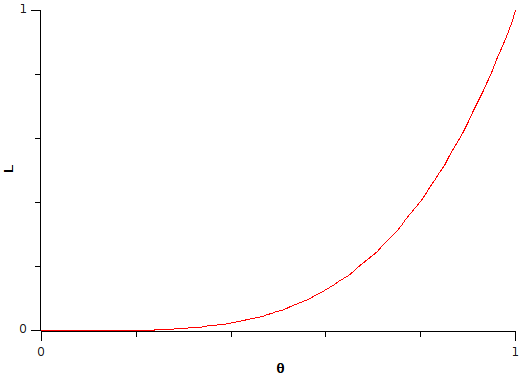
\includegraphics[scale=0.5]{img/verosim.png}
      \caption{Andamento della verosimiglianza\label{fig:verosim1}}
  \end{figure}

La verosimiglianza, come si vede in figura \ref{fig:verosim1}, raggiunge il suo massimo valore nel secondo caso, ovvero per $\theta=1$, il che significa che siamo portati a pensare che la moneta sia truccata e che dia sempre testa.
\end{esempio}

\begin{esempio} %###########
Usiamo ancora la stessa moneta dell'esempio precedente ed otteniamo un differente insieme di dati $\bar{x}=\{T,T,C,C\}$ e quindi la verosimiglianza diventa:

    \[ L(\bar{\theta},\bar{x})=L(\theta,\{T,T,C,C\})=P(\{T,T,C,C\}|\theta)=\theta \cdot \theta \cdot (1-\theta) \cdot (1-\theta) = \theta^2 \cdot (1-\theta)^2 \]

valutiamola quindi per alcuni valori di $\theta$:

\begin{enumerate}
  \item $\theta=1  \Rightarrow L(\theta,x)=\theta^2 \cdot (1-\theta)^2=1 \cdot 0=0$
  \item $\theta=\frac{1}{2}  \Rightarrow L(\theta,x)=\theta^2 \cdot (1-\theta)^2=0.25 \cdot 0.25=0.0625$
  \item $\theta=\frac{1}{10}  \Rightarrow L(\theta,x)=\theta^2 \cdot (1-\theta)^2=0.01 \cdot 0.081=0.0081$
\end{enumerate}

  \begin{figure}[htbp]
    \centering
    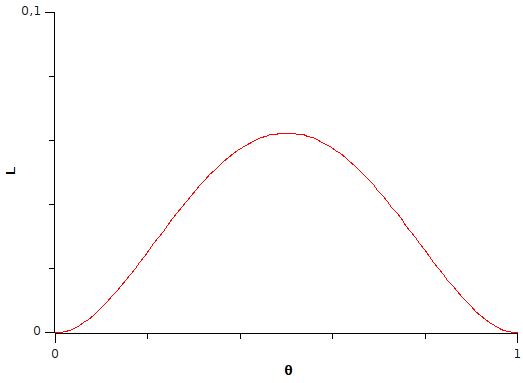
\includegraphics[scale=0.5]{img/verosim2.png} 
    \caption{verosimiglianza\label{fig:verosim2}}
  \end{figure}
La massima verosimiglianza, come si vede in figura \ref{fig:verosim2}, è raggiunta nel secondo caso, per $\theta=\frac{1}{2}$, il che significa che siamo portati a pensare che la moneta sia onesta e che mediamente esca testa la metà delle volte.
\end{esempio}

Dagli esempi si evince che il parametro $\theta$ di cui vogliamo una stima con il criterio della massima verosimiglianza, è dato dal valore che massimizza la funziona di verosimiglianza, quindi:

    \[ \theta^{ML}(X)=\arg \max_{\theta \in D_\theta} L(\theta,X) \]

Da notare che la funzione di verosimiglianza $L$ non è una ddp, ciò che varia è $\theta$ e non $X$, infatti $\theta$ non è nemmeno una V.C. ma un risultato puntuale di una funzione, inoltre, non essendo una V.C:

  \[ \int_{D_\theta}^{}L(\theta,X) d\theta\ne 1 \]
  
Molto spesso massimizzare la verosimiglianza può essere computazionalmente complesso e quindi può essere utile risolvere il problema di massimizzazione del supporto della verosimiglianza\index{Supporto della verosimiglianza}\index{Log likelihood}; ai fini della stima del parametro $\theta$ i metodi sono equivalenti. Definiamo allora il supporto della verosimiglianza (Log likelihood):

  \[ S(\theta,X):= \ln L(\theta,X)  \]
  
e quindi la stima ML diventa:

  \[ \theta^{ML}(X)=\arg \max_{\theta \in D_\theta} S(\theta,X)  \]
  
Un esempio piuttosto comune che rende preferibile la massimizzazione del supporto è dato dall'uso di V.C. iid. Il motivo è che la ddp congiunta di V.C. iid è la produttoria di tutte le ddp, quindi in fase di massimizzazione il calcolo della derivata diventa complesso:

  \[ L(\theta,X)=f_X^{(\theta)}(x)=\prod_{i=1}^{N}  f_{X_i}^{(\theta)}(x)  \]
  
con l'uso del supporto la massimizzazione diventa molto più semplice, infatti:

  \[ S(\theta,X)= \ln L(\theta,X )= \ln \prod_{i=1}^{N}  f_{X_i}^{(\theta)}  =  \sum_{i=1}^{N}   f_{X_i}^{(\theta)} \]
  
Concludiamo con alcune proprietà di cui gode lo stimatore ML. Sotto ipotesi di regolarità, lo stimatore ML, per campioni indipendenti, è uno stimatore asintoticamente: consistente, gaussiano e non polarizzato, inoltre, sempre asintoticamente, raggiunge il limite CR. Ovviamente queste proprità non valgono per piccole quantità di dati.
Sempre sotto ipotesi di regolarità vale:

  \[ \eta = h(\theta^{ML}) \]

\begin{esempio}  
Supponiamo di voler stimare una valore $x^3$, allora:

  \[ h(x)=x^3 \]
  
e quindi possiamo stimare $\theta^{ML} = x$ e poi calcolare:

  \[ \eta^{ML} = h(\theta^{ML})={\theta^{ML}}^3 \]
\end{esempio}

In conclusione, possiamo affermare che la stima ML ha il grande pregio di essere una tecnica molto generale, ma ha un difetto altrettanto grande che dipende dalla conoscenza della ddp congiunta dell'esperimento, il che è difficilmente noto a priori.

  % stima a posteriori
  \section{Stima a posteriori} 
% ######################################################################## Introduzione
\subsection{Introduzione}
\index{Stima a posteriori}Al contrario di ciò che avviene per la stima ML, nella stima a posteriori descriviamo il parametro $\theta$ come una V.C. (Teorema di Bayes). Questo criterio di stima si basa sulle conoscenze a priori che si hanno sull'esperimento, ovvero tutte quelle conoscenze che già abbiamo circa l'esperimento osservato. In figura \ref{fig:apriori1} e \ref{fig:apriori2} vediamo alcuni esempi di conoscenze a priori:

\begin{figure}[!p]
  \centering
        \subfigure
        [sappiamo che $\theta$ assume un valore nell'intervallo $a,b$ senza nessuna preferenza\label{fig:thetaAB}]
        {\includegraphics[keepaspectratio]{mathematica/prior1}}
  
        \subfigure
        [sappiamo che $\theta$ tende, in media, ad assumere il valore $\bar{\theta}$ (con più o meno incertezza)\label{fig:thetagauss}]
        {\includegraphics[keepaspectratio]{mathematica/prior2}}
        \caption{esempi di conoscenze a priori.\label{fig:apriori1}}
\end{figure}
\begin{figure}[p]
  \centering  
        \subfigure
        [sappiamo che $\theta=\bar{\theta}$\label{fig:thetaexact}]
        {\includegraphics[keepaspectratio]{mathematica/prior3}}
  
        \subfigure
        [sappiamo che $\theta \geq 0$ ma che i valori alti sono via via meno probabili\label{fig:thetaexp}]
        {\includegraphics[keepaspectratio]{mathematica/prior4}}
  
  \caption{esempi di conoscenze a priori.\label{fig:apriori2}}
\end{figure}

Modifichiamo ora il nostro diagramma del problema di stima di modo che sia presente anche questa conoscenza a priori. Come si vede in figura \ref{fig:diagrammastima2} il nuovo elemento introdotto $\Sigma_1$ è la sorgente casuale caratterizzata dalla ddp della conoscenza a priori $f_\Theta(\theta)$; in questo modo $\Sigma$ sarà caratterizzata da una ddp che subisce una dipendenza $f_{X|\Theta}(X|\Theta=0)$.
\begin{figure}[h]
  \centering
  \[
    \begin{CD}
     \framebox{$\theta^0$} @>>> \framebox{$\Sigma_1, f_\Theta(\theta^0)$} @>>>  \framebox{$\Sigma, f_{X|\Theta}(X|\Theta=0)$} @>X>> \framebox{$g(X)$} @>>> \framebox{$\hat{\theta}$}
    \end{CD}
  \]
  \caption{Diagramma di stima\label{fig:diagrammastima2}}
\end{figure}
L'idea alla base della stima a posteriori è che se conosciamo $f_{\Theta}(\theta)$ e $f_{X|\Theta}(X|\Theta=0)$, possiamo calcolare la ddp a posteriori  condizionata dal vettore delle osservazioni $X$, mediante il teorema di Bayes\index{Teorema di Bayes}:

  \[ f_{\Theta|X}(\theta|X)=\frac{f_{X|\Theta}(X|\theta) \cdot f_\Theta(\theta)}{\int_{D_\theta}^{} f_{X|\Theta}(X|\theta) \cdot f_\Theta(\theta) d\theta } \]
  
Vediamo ora alcuni esempi per meglio chiarire la stima a posteriori.

\begin{esempio}
Sia data una scatola di monete: il 40\% sono oneste, il rimanente 60\% sono truccate. Per le monete truccate la probabilità che esca testa è dell'80\% $P(T)=0.8$ . Estraendo una moneta a caso: qual'è la probabilità che sia truccata? Se dopo averla lanciata esce croce: qual'è la probabilità, a posteriori, che sia una moneta truccata?\newline
La conoscenza a priori di questo esperimento è dato dalla conoscenza della quantità di monete truccate presenti:
[manca la graffa grossa tipo sistema $\Theta \{$]

  \begin{align*}
    0 \rightarrow &P(\Theta=0)=0.4 \\ 
    1 \rightarrow &P(\Theta=0)=0.6
  \end{align*}
  
Ora vediamo le probabilità condizionate, sapendo che dal lancio è uscita croce $(C)$:

  \begin{align*}
    &P(C|\theta=0)=0.5 \quad \text{ sapendo che la moneta è onesta}\quad &P(C)=0.5 \\
    &P(C|\theta=1)=0.2 \quad \text{ sapendo che la moneta è truccata}\quad &P(C)=0.2
  \end{align*}
  
Da questi due ultimi dati osserviamo che: se dal lancio è uscito croce, la probabilità che la moneta sia truccata è molto bassa perché nel caso in cui la moneta sia truccata, la probabilità che esca croce è 0.2. Infatti, valutando la probabilità a posteriori otteniamo proprio questo risultato:


    \[ P(\theta=1|C)=\frac{P(C|\theta=1) \cdot P(\theta=1)}{P(C|\theta=1) \cdot P(\theta=1) + P(C|\theta=0) \cdot P(\theta=0)}=0.375 \]

%FIXME
\textbf{[grafici pre e post lancio]}
\end{esempio}

\begin{esempio}
Sia data una moneta di cui non si conosce nulla, si vuole stimare $p=P(T)$.\newline
Non avendo alcuna informazione sulla moneta, non conosciamo se sia onesta o truccata né quindi "quanto" truccata, quindi la nostra conoscenza a priori è inesistente.\newline
Dato che non abbiamo informazioni a priori, prima di effettuare l'esperimento la nostra stima di $p=P(T)$ è del tutto indifferente sull'onestà della moneta, quindi non emerge alcuna preferenza nella ddp.

%FIXME grafico dell'indifferenza
\begin{center}\textbf{[grafico dell'indifferenza]}\end{center}

Iterando il processo, ed aggiornando la ddp, un numero di volte sufficiente si tende ad ottenere la stima esatta.

%FIXME grafici delle iterazioni
\textbf{[grafici di iterazione]}
\end{esempio}

Giunti a questo punto ci si pone un problema: conoscendo $f_{\theta|X}(\theta|X)$ come scelgo il valore dello stimatore $\hat{\theta}$? Come abbiamo visto per la stima ML, si sceglieva il valore che massimizzava la ddp congiunta; ma in questo caso qual'è il valore "migliore" da scegliere? Potremmo scegliere la media, la moda o anche la mediana. Quello che occorre è un metodo per scegliere correttamente il valore.\newline
Una buona idea potrebbe essere quella di valutare l'errore quadratico e quindi scegliere il valore che lo minimizza.
\paragraph{Teorema} $J:=E[(X-\hat{x})^2]$ è minimo se e solo se $\hat{x}=E[X]$
ovvero, il valore atteso dell'errore quadratico è minimo in corrispondenza del valore atteso del campione.

\begin{dimostrazione}
Sapendo che possiamo calcolare il valore atteso di una V.C. $Y$ linearmente dipendente da un altra $X$ senza conoscere direttamente la sua ddp $f_Y(y)$ come:

  \[ E[Y]=E[g(x)]=\int_{-\infty}^{\infty} {g(x) \cdot f_X(x)dx}  \]
allora possiamo anche scrivere:

  \[ J=E\left[ (X-\hat{x})^2\right] = \int_{-\infty}^{ \infty }  {(X-\hat{x})^2 \cdot f_X(x) \cdot dx} \]
Volendo ora minimizzare l'errore quadratico calcoliamo il punto (i punti) in cui la sua derivata prima si annulla:

  \[ \begin{split}
      \frac{\partial J}{\partial\hat{x}}=0 & \Leftrightarrow  \int_{-\infty}^{ \infty }  {2(X-\hat{x}) \cdot f_X(x) \cdot dx}=0  \Leftrightarrow \\
      & \Leftrightarrow \int_{-\infty}^{ \infty }  {X \cdot f_X(x) \cdot dx}=\int_{-\infty}^{ \infty }  {\hat{x} \cdot f_X(x) \cdot dx}  \Leftrightarrow \\
      & \Leftrightarrow \hat{x}=\int_{-\infty}^{ \infty }  {X \cdot f_X(x) \cdot dx} = E[X]
    \end{split} 
  \]
  
Come volevasi dimostrare l'errore quadratico ha il suo punto di minimo in corrispondenza del valore atteso di $X$.
\end{dimostrazione}
Ne concludiamo che se volessimo minimizzare l'errore quadratico è opportuno scegliere la media come punto di riferimento. Se, invece, avessimo voluto minimizzare l'errore  è dimostrabile che il valore ottimo è dato dalla mediana.
% ########################################################################
\subsection{Stima di una variabile casuale in funzione di un'altra variabile casuale}
Un problema molto ricorrente nei problemi di stima è quello di fornire una stima per una V.C. usando informazioni provenienti da altre V.C., ad esempio potremmo misurare l'altezza di un campione di persone e stimarne il peso. Ovviamente non è sempre possibile fare una stima di una V.C. in funzione di altre V.C.: il requisito fondamentale per rendere sensata la stima è che le V.C. in oggetto $X,Y$ siano correlate e che la loro ddp congiunta $f_{XY}(x,y)$ sia nota. Chiaramente non possiamo pensare di stimare il peso di una persona in funzione della temperatura atmosferica perché sono due V.C. non correlate. Dato che conosciamo $f_{XY}(x,y)$ allora conosciamo anche:

  \[ f_{X|Y}(x,y) = \frac{f_{XY}(x,y)}{f_Y(y)}= \frac{f_{XY}(x,y)}{\int_{-\infty}^{\infty} f_{XY}(x,y)dx} \]
  
e quindi, essendo nota anche $Y$, tutto ciò che sappiamo di $X$ è riassunto nella ddp condizionata $f_{X|Y}(x,y)$. Come per il teorema dimostrato nel capitolo precedente, anche in questo caso c'è un teorema analogo, anch'esso dimostrabile nello stesso modo del precedente (con i dovuti accorgimenti).

\paragraph{Teorema} $E\left[(X-\hat{X}(y))^2|Y=y\right]$ è minimo se e solo se $\hat{X}=E[X|Y=y]$
 è minimo 
ovvero, che il valore atteso per l'errore quadratico condizionato da $Y$ è minimo in corrispondenza del valore atteso di $X$ condizionato da $Y$.\newline
Questo che abbiamo risolto è il problema di stima in media quadratica - Mean Square (MS) \index{Stima Mean Square (MS)}. Possiamo fare alcune considerazioni su quanto detto in questo capitolo:
\paragraph{Osservazione 1} Se $X$ e $Y$ sono indipendenti, quindi incorrelate, allora la conoscenza di una non aiuta a determinare l'altra, infatti:

  \begin{gather*}
    E[X|Y=y]=E[X] \\
    E\left[(X-\hat{X}(y))^2|Y=y\right]=E\left[(X-E[X])^2\right]=Var[X]
  \end{gather*}
  
\paragraph{Osservazione 2} Se $X$ e $Y$ sono congiuntamente gaussiane (anche nel caso vettoriale), sappiamo che:
  \[ \hat{X}(y)=E[X|Y=y]=E[X]+cov(X,Y) \cdot \frac{1}{Var[Y]} \cdot (Y-E[Y]) \]
ricordandoci della definizione del coefficiente di correlazione:
  \[ r_{XY}=\frac{cvo(X,Y)}{\sqrt{Var[X]Var[Y]} }=\frac{\sigma_{XY}}{\sigma_X\sigma_Y} \]
riscrivendo l'equazione precedente:
  \[ \frac{\hat{X}(y)-E[X]}{\sigma_X}=r_{XY}\frac{Y-E[Y]}{\sigma_Y} \]
il termine di sinistra rappresenta una pseudo standardizzazione del parametro (essendo stimato non è una vera standardizzazione), il termine di destra, oltre il coefficiente di correlazione, è la standardizzazione di $Y$. Come si può notare fra i parametri standardizzati c'è una relazione lineare che dipende dal coefficiente di correlazione.\newline
Sempre nel caso di gaussianità congiunta:

  \[ 
    \begin{split}
    E\left[(X-\hat{X}(y))^2\right] & =Var[(X-\hat{X})|Y=y]=\sigma_x^2-\frac{\sigma_{XY}^2}{\sigma_Y^2}\\
    & =\sigma_X^2(1-\frac{\sigma_{XY}^2}{\sigma_X^2\sigma_Y^2})=\sigma_{XY}^2(1-r_{XY}^2) 
    \end{split}
  \]
  
distinguiamo ora i due casi estremi, di cui la figura \ref{fig:confrontomaxminr} ne da una rappresentazione:

  \begin{align*}
    r_{XY}&=0    &\Rightarrow\quad &Var\left[(X-\hat{X})^2|Y=y\right]=\sigma_X^2  &\text{ non c'è correlazione} \\
    r_{XY}&=\pm1 &\Rightarrow\quad &Var\left[(X-\hat{X})^2|Y=y\right]=0  &\text{ la correlazione è massima}
  \end{align*}
  
  \begin{figure}[htbp]
    \centering
    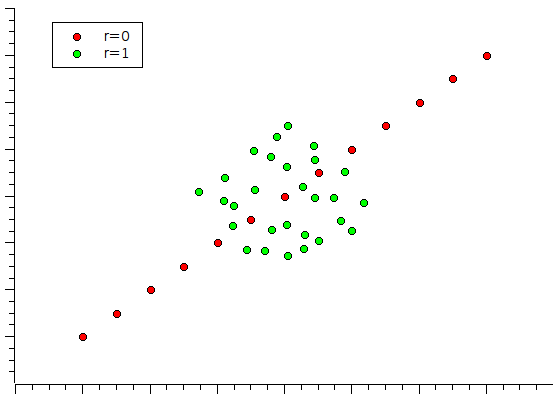
\includegraphics[scale=0.5]{img/correlazione.png}
    \caption{confronto fra correlazione massima e minima\label{fig:confrontomaxminr}}
  \end{figure}
  
Nel caso gaussiano $\hat{X}(y)$ è una funzione lineare di $y$, inoltre, l'errore quadratico medio $E\left[(X-\hat{X}(y))^2|Y=y\right]$ non dipende da $y$: la qualità della stima la conosciamo già prima di avere le osservazioni.\newline
Nel caso più generale (non gaussiano) lo stimatore MS è una funzione non lineare di $y$. Trattando vettori di V.C. congiunte e gaussiani abbiamo:

  \begin{align*}
    Var\begin{bmatrix} X \\ Y\end{bmatrix} &=\begin{bmatrix} V_{XX} & V_{XY} \\ V_{YX} & V_{YY} \end{bmatrix}=\begin{bmatrix} Var[X] & cov[X,Y] \\ cov[Y,X] & var[Y]\end{bmatrix} \\
    E[X|Y=y]&=E[X]+V_{XX} \cdot V_{YY} \cdot (y-E[Y]) \\
    Var\left[(X-\hat{X}|Y=y)\right]&=V_{XX}-V_{XY} \cdot V_{YY}^{-1} \cdot V_YX
  \end{align*}
  
Come abbiamo visto la linearità è solo un caso particolare della gaussianità congiunta, lo stimatore MS è generalmente non lineare e quindi di più difficile trattazione, sia teorica che computazionale. In figura \ref{fig:confrontogaussgenerico} è rappresentato un esempio di angamento gaussiano e un andamento generico.

  \begin{figure}[htbp]
    \centering
    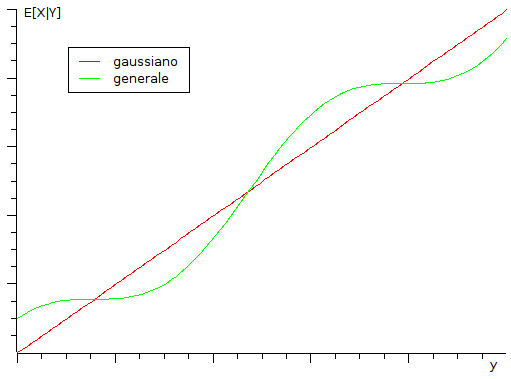
\includegraphics[scale=0.5]{img/gaussgeneral.png}
    \caption{confronto fra il caso gaussiano e quello generico\label{fig:confrontogaussgenerico}}
  \end{figure}

Avere a che fare con problemi lineari è molto più comodo, quindi, anche se il modello ideale è di tipo non lineare vogliamo quindi restringerci alla sola classe degli stimatori lineari - stimatore MS lineare- :

  \[ \hat{X}_L(y)=aY+b \]
  
\paragraph{Teorema} l'errore:

  \[ J=E\left[(X-\hat{X}_L(y))^2\right]=E\left[(X-aY-b)^2\right] \]
  
è minimizzato in corrispondenza di:

  \[ \hat{X}_L(y)=E[X|Y=y]=E[X]+cov(X,Y) \cdot \frac{1}{Var[Y]} \cdot (Y-E[Y])\]
  
Altro non è che la stessa formula del caso gaussiano. Nel caso vettoriale, invece:

  \begin{gather*}
    \hat{X}_L(y)=E[X]+V_{XX} \cdot V_{YY}^{-1} \cdot (Y-E[Y]) \\
    E\left[(X-\hat{X}_L(y))\cdot (X-\hat{X}_L(y))^T\right]=V_{XX}-V_{XY} \cdot V_{YY}^{-1}  \cdot V_{YX}
  \end{gather*}
  
Lo stimatore MS lineare è l'ottimo assoluto nel caso gaussiano, nel caso non gaussiano è ancora ottimo ma limitatamente alla classe degli stimatori lineari.
% ########################################################################
\subsection{Stimatori a posteriori}
Partiamo dal presupposto di aver calcolato, o di conoscere già, la ddp condizionata $f_{\Theta|X}(\theta|X)$ \footnote{ovvero i parametri in funzione dei dati}, come calcoliamo la stima $\hat{\theta}$? Per fare ciò abbiamo diverse alternative
\subsubsection{Stima Maximum A Posteriori - MAP}  %############
\index{Stima maximum a posteriori (MAP)}
  \[ \theta^{MAP}(X)=\arg \max_\theta f_{\Theta|X}(\theta|X) \]
  
Il valore del parametro stimato $\hat{\theta}$ è individuato in corrispondenza della moda della ddp a posteriori.
Per il teorema di Bayes, enunciato precedentemente, il denominatore è un valore indipendente dal parametro $\theta$, quindi non concorre alla determinazione del valore che massimizza la ddp a posteriori:

  \[ f_{\Theta|X}(\theta|X)=\frac{f_{X|\Theta}(X|\theta) \cdot f_\Theta(\theta)}{...} \]
  
quindi possiamo anche scrivere:

  \[ \theta^{MAP}(X)=\arg \max_\theta f_{X|\Theta}(X|\theta) \cdot f_\Theta(\theta) \]
  
Confrontando quest'ultima formulazione della stima MAP notiamo che assomiglia molto alla stima ML, infatti, senza conoscenza a priori sarebbe la formula della verosimiglianza, ma anche nel caso in cui la conoscenza a priori sia uniforme, ovvero $f_\Theta$ è costante.\newline
Come per la stima ML, anche per la stima MAP poterebbe essere più conveniente massimizzare il supporto, inoltre, tutte le tecniche di calcolo numerico adottate per la stima ML sono ancora valide per la stima MAP (di cui la stima ML è un caso particolare).
Come abbiamo visto, la stima MAP usa la moda come parametro di riferimento, ma con alcuni tipi di distribuzione la moda è poco significativa, ad esempio quando la ddp a posteriori è di tipo esponenziale come in figura \ref{fig:expMAP}, si avrebbe $\theta^{MAP}=0$ quando, invece, è ben evidente che c'è il 100\% di probabilità che ciò non sia vero, ma che $\theta^{MAP}>0$

\begin{figure}[htbp]
  \centering
  \includegraphics[scale=1]{mathematica/esponenziale}
  \caption{esponenziale\label{fig:expMAP}}
\end{figure}


\subsubsection{Stima di Bayes - B} %############
\index{Stima di Bayes}
  \[ \theta^B(X)=E[\Theta|X] \]
è lo stimatore in media quadratica. Se $\Theta$ e $X$ sono congiuntamente gaussiane, allora:

  \begin{gather*}
    \theta^B(X)=\theta^{MAP}(X)=E[\Theta]+V_{\Theta X} \cdot V_X^{-1} \cdot (X-E[X])\\
    Var \left[\begin{bmatrix} X \\ \Theta \end{bmatrix} \right]=\begin{bmatrix} V_X \ V_{X\Theta} \\ V_{\Theta X}^T \ V_\Theta \end{bmatrix}
  \end{gather*}
  
Nei casi in cui, invece, non siano congiuntamente gaussiane è raro trovare formulazioni esplicita; questo spiega il successo della stima MAP, infatti, risulta molto più facile risolvere un problema di massimizzazione piuttosto che risolvere l'integrale che richiede la stima di Bayes. Un'altro punto debole della stima di Bayes risiede proprio nell'uso del valore medio, infatti, nei casi in cui la scelta è vincolata a valori discreti la stima di Bayes potrebbe ritornare un valore inesistente, ad esempio: supponendo di avere una moneta e di stimare se è onesta ($\Theta=0$) o truccata ($\Theta=1$) con $p=0.8$, la stima di Bayes risulterebbe $\theta^B=0.2$, che è un risultato senza significato perché noi volevamo una stima sull'onesta: o lo è, o non lo è.
\subsubsection{Stima Mean Square lineare - MS} %############
\index{Stima Mean Square lineare (MS)}
  \[ \theta^{MS}(X)=E[\Theta]+V_{\Theta X} \cdot V_X^{-1} \cdot (X- E[X]) \]
Nel caso in cui $\Theta$ e $X$ siano congiuntamente gaussiani, lo stimatore MS coincide con lo stimatore di Bayes ma anche con lo stimatore MAP, infatti, nel caso gaussiano gli stimatori sono tutti uguali perché media, moda e mediana cadono nello stesso punto.
\subsubsection{Stimatore mediano} %###########

  \[ \hat{\theta}=mediana(f_{\Theta|X}) \]
  
Questo stimatore può avere dei vantaggi rispetto allo stimatore con media perché se vi sono degli outlier molto grandi la media viene influenzata di molto, mentre la mediana no.
% ######################################################################## Conclusioni
\subsection{Conclusioni}
Come conclusione della stima a posteriori cerchiamo di capire quando è utile usarla.

  \begin{itemize}
    \item se il parametro da stimare $\theta$ è una V.C. (ad esempio l'estrazione da una scatola di monete oneste o truccate) 
    \item stima sequenziale, ovvero i dati arrivano dilazionati nel tempo. All'inizio si ha un insieme di dati e si costruisce una prima stima, con l'arrivo di altri dati bisogna ricostruire la stima. Si può procedere in due modi: mettere insieme tutti i dati e rifare la stima; oppure, propagare l'informazione usando la prima stima come stima a priori ed elaborarla assieme ai nuovi dati usandoli come stima a posteriori. 
    \item usiamo $f_{\Theta}$ come conoscenza a priori, questo ha il vantaggio di essere più generale della stima ML e di ottenere risultati anche con pochi dati; di contro si fanno ipotesi molto forti e il problema della scelta della funzione $f_{\Theta}$ 
  \end{itemize}

  % intervalli di confidenza
  \section{Intervalli di confidenza}
\index{Intervallo di confidenza}
Fare delle stime senza dare alcuna indicazione sulla loro precisione può essere poco significativo e/o addirittura fuoriviante, ad esempio:

%FIXME fare i grafici
  \begin{figure}[htbp]
    \centering
    %\includegraphics[scale=0.6]{img/grafIntConf.png}
    \caption{Grafici di intervalli di confidenza \label{fig:grafIntConf}}
  \end{figure}
Come si vede dai grafici in figura \ref{fig:grafIntConf}, nel primo caso abbiamo una stima che potrebbe cadere in un intervallo molto ampio, quindi è meno affidabile della stima del secondo caso, dove l'intervallo è più stretto.\newline
Data una stima è desiderabile che questa cada all'interno di un intervallo piccolo. Con il valore $\gamma$ indichiamo il livello di confidenza della stima, ovvero la probabilità che la stima cada in un certo intervallo.


\begin{esempio} % ###########
Avendo a disposizione la stima a posteriori con ddp unimodale e simmentrica, con $\gamma=0.9$ abbiamo il 90\% di probabilità di cadere dell'intervallo $I_{0.9}=[\theta^B-\sigma \cdot 0.9 ; \theta^B + \sigma \cdot 0.9]$ \newline
[grafico]\newline
L'intervallo che abbiamo definito è detto intervallo di confidenza al 90\%
\end{esempio}

Sia dato uno stimatore $\hat{\theta}$ gaussiano non polarizzato avente varianza nota; risolviamo ora il problema di trovare il suo intervallo di confidenza $I_\gamma$ dato $\gamma$. Per risolvere il problema è utile standardizzare con una gaussiana standard e quindi calcolare:

  \[ Z=\frac{\hat{\theta}-\theta}{\sigma_{\hat{\theta}}}\sim G(0,1) \]
  
Ora, utilizzando le tabelle della gaussiana standard, troviamo:

  \[  z_0 | P(-z_o \leq Z \leq z_0)=P(\left| Z \right| \leq z_0 )=\gamma \]
  
  \[ 
    \begin{split}
      F_Z(z_0)-F_Z(-z_0) & =F_Z(z_0)-(1-F_Z(z_0))=2F_Z(z_0)-1=\gamma \Rightarrow \\
      F_Z(z_0) & =\frac{1+\gamma}{2} \Rightarrow P\left(\left| \frac{\hat{\theta}-\theta}{\sigma_{\hat{\theta}}} \right| \leq z_0 \right)=\gamma \Rightarrow \\
      P\left(\left| {\hat{\theta}-\theta}\right|\leq z_0\cdot \sigma_{\hat{\theta}} \right) & =\gamma\Rightarrow P(\hat{\theta}-z_0\cdot\sigma_{\hat{\theta}}\leq\theta\leq\hat{\theta}+z_0 \cdot\sigma_{\hat{\theta}})=\gamma \Rightarrow \\
      I_\gamma & =\left[\hat{\theta}-z_0\cdot\sigma_{\hat{\theta}} \quad,\quad\hat{\theta}+z_0\cdot\sigma_{\hat{\theta}}\right]
    \end{split}
  \]
  
Quello che abbiamo appena trovato è l'intervallo di confidenza, ovvero l'intervallo dove cade il $\gamma\%$ di probabilità; per trovarlo siamo partiti cercando un valore $z_0$ tale che la probabilità che i valori fossero compresi fra $\pm z_0$ fosse pari a $\gamma$.\newline
Secondo la scuola Bayesiana questo è un imbroglio perché $\theta$ non è una V.C. ma un numero ben definito che andiamo a calcolare in modo puntuale. L'imbroglio sta nel dire che $\theta \in I_\gamma$ perché una volta raccolti i dati $\hat{\theta}$ è un numero puro e non ha quindi alcuna variabilità, caratteristica tipica delle V.C. . In difesa del metodo vi è l'osservazione che ripetendo l'esperimento, e quindi ottenendo nuovi dati, $\hat{\theta}$ potrebbe cambiare e quindi è trattabile come una V.C.


\begin{esempio} % ###########
Siano date $N$ $X_i$ V.C. iid con $Var[X_i]=\sigma^2$, $\sigma^2$ nota ed $N$ grande. Trovare l'intervallo di confidenza $I_\gamma$ per $M_1$.\newline
Il parametro che dobbiamo cercare è $\theta=m$. Conosciamo già una stimatre della media, ovvero la media campionaria, quindi:
 
 \begin{gather*}
    \hat{\theta}=M_1 \\
    \sigma_{\hat{\theta}}=\sqrt{\frac{\sigma^2}{N}}=\frac{\sigma}{\sqrt{N}}
 \end{gather*}
 
dato che $N$ è grande, per il teorema del limite centrale, $M_1 \sim G(m,\frac{\sigma}{\sqrt{N}})$. Possiamo quindi scrivere l'intervallo di confidenza come:

  \[ I_\gamma = \left[ M_1-z_0\frac{\sigma}{\sqrt{N}} \quad ,\quad M_1+z_0\frac{\sigma}{\sqrt{N}} \right]  \]
\end{esempio}
\begin{esempio} % ###########
Siano dati $N=100$ campioni, $\gamma=0.9$ : calcolare l'intervallo di confidenza $I_\gamma$.

  \[ \frac{1+\gamma}{2}=0.95 \Longrightarrow F(z_0)=0.95 \]
  
Dalle tabelle cerchiamo ora $z_0 | F(z_0)=0.95$:

  \[ z_0=1.645 \Longrightarrow I_{0.9}=\left[ M_1-1.645\frac{\sigma}{10} \quad ,\quad M_1+1.645\frac{\sigma}{10} \right]  \]
\end{esempio}
\begin{esempio} % ###########
Siano dati $N=100$ campioni e l'intervallo di confidenza $I_\gamma=\left[ M_1-\delta \quad ,\quad M_1+\delta \right[ $: calcolare $\gamma$.\newline
Ipotizzando che $\delta=z_0\frac{\sigma}{\sqrt{N}}$ possiamo calcolare $z_0=\frac{\delta\sqrt{N}}{\sigma}$. A questo punto dalle tabelle possiamo ricavare il valore di $F(z_0)$, quindi risolvendo la seguente equazione troviamo $\gamma$:

  \[ F(z_0)=\frac{1+\gamma}{2} \Longrightarrow \gamma= 2F(z_0)-1 \]
\end{esempio}
\begin{esempio} % ###########
Sia dato l'intervallo di confidenza $I_\gamma=\left[ M_1-\delta \quad ,\quad M_1+\delta \right] $, con $\gamma=0.95$: calcolare il numero di campiono $N$. In pratica il problema si può esprimere anche nel seguente modo: quanti campioni occorre raccogliere perché si cada al 95\% dentro all'intervallo di confidenza $I_{0.95}$ ?\newline
Innanzi tutto possiamo ricavare $z_0$:

  \[ F(z_0)=\frac{1+\gamma}{2}=0.975 \Longrightarrow z_0=1.96 \]
  
Supponendo poi che $\delta=z_0\frac{\sigma}{\sqrt{N}}$, possiamo calcolare $N$ come:

  \[ \delta=z_0\frac{\sigma}{\sqrt{N}} \Longrightarrow N=z_0^2\left( \frac{\sigma}{\delta}\right) ^2 \]
  
Da notare che la precisione è molto costosa, infatti, se volessimo un $\delta$ piccolo in numero di campioni $N$ necessario cresce rapidamente:

\[ \lim_{\delta \rightarrow 0} {N}=\infty \]
\end{esempio}


Quello che abbiamo fatto fin ore è far riferimento ad una standardizzazione con una gaussiana; un'alternativa, utile per piccoli campioni, è la $t$ di Student, definita come:
\[ T_N:=\frac{Z}{\sqrt{\sum_{i=1}^{N}Z_i^2}} \cdot \sqrt{N}=\frac{Z}{\chi_N} \cdot \sqrt{N} \]
dove $Z$ e $Z_i$ sono V.C. iid $\sim G(0,1)$; $T_N$ è detta $t$ di Student a $N$ gradi di libertà, ed ha un andamento come in figrua \ref{fig:grafIntConfTstud}:
  \begin{figure}[htbp]
    \centering
    %\includegraphics[scale=0.6]{img/grafIntConf.png}
    \caption{Grafici di intervalli di confidenza \label{fig:grafIntConfTstud}}
  \end{figure}
L'andamento è simile ad una gaussiana, ma con una varianza maggiore. Per la $t$ di Student valgono le seguenti proprietà:

  \begin{gather*}
    E[T_N]\\
    Var[T_N]=\frac{N}{N-2}\\
    \lim_{N\rightarrow \infty} T_N = G(0,1)
  \end{gather*}


% IDENTIFICAZIONE DEI MODELLI STATICI
\chapter{Identificazione dei modelli statici}
  %introduzione
  \section{Introduzione}
Con l'identificazione dei modelli vogliamo trovare un modello matematico (una funzione) che leghi, nel miglior modo possibile, un'insieme di dati riguardanti variabili indipendenti con un'insieme di dati dipendenti.

\begin{figure}[htbp]
  \centering
  \[
    \begin{CD}
       @>u>> \framebox{$Y=\Phi(u,\theta)$} @>Y>>
    \end{CD}
  \]
  \caption{Diagramma di un modello statico\label{fig:diagrammamodstat}}
\end{figure}

\begin{itemize}
    \item $Y$ è l'insieme delle variabili dipendenti, ovvero i dati misurati sull'esperimento che vogliamo spiegare con un modello
    \item $u$ è l'insieme delle variabili indipendenti, ovvero dati misurati, o noti a priori, mediante i quali voglio spiegare gli effetti
    \item $\Phi( , )$ è il modello matematico che lega $u$ ad $Y$
    \item $\theta$ parametri incogniti del modello
\end{itemize}

\begin{esempio} % ###########
Per chiarire il concetto di identificazione del modello, prendiamo, ad esempio, una resistenza di cui conosciamo differenza di potenziale $V$ e corrente $I$ e vogliamo trovare il modello che permette di determinare la corrente in funzione della differenza di potenziale.
\begin{figure}[htbp]
  \centering
  \includegraphics[ scale=0.5]{img/resistenza}
  \caption{Schema circuitale di una resistenza\label{fig:resistenza}}
\end{figure}

Dopo alcune misure sperimentali otteniamo:

\begin{figure}[htbp]
  \centering
  \includegraphics[ keepaspectratio]{mathematica/resistenza}
  \caption{In figura è rappresentato l'andamento del modello, confrontato con l'andamento reale del sistema. Presi alcuni campioni si nota l'esistenza di un errore $\varepsilon$ nel modello rispetto alla realtà\label{fig:modelloresistenza}}
\end{figure}

La retta rappresentata nel grafico nella realtà non si verifica mai per via di errori di misura, inoltre, la relazione perfettamente lineare sussiste solo nel caso di una resistenza ideale.
Nel caso di questo esempio la variabile dipendente è la corrente, quindi $Y=I$, mentre la variabile indipendente è la differenza di potenziale, quindi $u=V$; ne consegue che il modello che vogliamo trovare sarà:

  \begin{align*}
    Y&=\Phi (u,\theta) \quad     u=\begin{bmatrix} V_1 \\ V_2 \\ \vdots \\ V_N\end{bmatrix} \quad  Y=\begin{bmatrix} I_1 \\ I_2 \\ \vdots \\ I_N \end{bmatrix}\\
    \theta&=R \vee \theta=\frac{1}{R}
  \end{align*}
  
Per la legge di Ohm sappiamo che la relazione che lega questi due valori è $I=\frac{V}{R}$, quindi il nostro modello sarà:

  \[ \Phi(u,\theta)=u \cdot \theta \vee \Phi(u,\theta)=u \cdot \frac{1}{\theta} \]
  
In questo caso abbiamo un modello lineare nei parametri.
\end{esempio}

\begin{esempio} % ###########
Supponiamo di conoscere la concentrazione plasmotica di un farmaco e che evolve secondo la legge:

  \[ C(t)=a \cdot e^{-\alpha t}+b \cdot e^{-\beta t} \]
  
i cui coefficienti $a$, $b$, $\alpha$, $\beta$ sono da stimare.
Sappiamo che il grafico di $C(t)$ ha un andamento esponenziale inverso, sappiamo, inoltre, che la concentrazione del farmaco è positiva e quindi $C(t)\geq 0$. Effettuano $N$ prelievi nel tempo otteniamo i campioni rappresentati in figura \ref{fig:concfarmaco}:

\begin{figure}[htbp]
  \centering
  \includegraphics[keepaspectratio]{mathematica/andamentofarmaco}
  \caption{Andamento della concentrazione di un farmaco nel sangue. Anche qua vediamo che il modello presenta degli errori rispetto all'andamento reale\label{fig:concfarmaco}}
\end{figure}

In questo caso il modello viene rappresentato in questo modo:

  \begin{align*}
    Y&=\begin{bmatrix} C(t_1)\\C(t_2)\\ \vdots \\ C(t_N) \end{bmatrix}\quad u=\begin{bmatrix} t_1 \\ t_2 \\ \vdots \\t_n \end{bmatrix}=\begin{bmatrix} u_1 \\ u_2 \\ \vdots \\u_n \end{bmatrix} \quad \theta=\begin{bmatrix} a \\ b \\ \alpha \\ \beta \end{bmatrix}=\begin{bmatrix} \theta_1 \\ \theta_2 \\ \theta_3 \\ \theta_4 \end{bmatrix}\\
    C(t_i)&=\theta_1 \cdot e^{-\theta_2 t_i} + \theta_3 \cdot e^{-\theta_4 t_i}
  \end{align*}
  
Da questo ne consegue che il nostro modello sarà:

  \[ \Phi(u,\theta)=\begin{bmatrix} \theta_1 \cdot e^{-\theta_2 t_1} + \theta_3 \cdot e^{-\theta_4 t_1}\\ \vdots  \\ \theta_1 \cdot e^{-\theta_2 t_N} + \theta_3 \cdot e^{-\theta_4 t_N} \end{bmatrix} \]
  
Questo è un esempio di modello non lineare nei parametri, infatti, i parametri $\theta_2$ e $\theta_4$ sono all'esponente, quindi non lineari. Ne consegue che non possiamo scrivere ilmodello come combinazione lineare.
\end{esempio}

\begin{esempio} % ###########
Prendiamo ora come esempio un campione di dati e cerchiamo di approssimare\footnote{mediante interpolazione} l'andamento dei punti con una funzione cubica, come in figura \ref{fig:andamentocubido}.

  \begin{figure}[htbp]
    \centering
    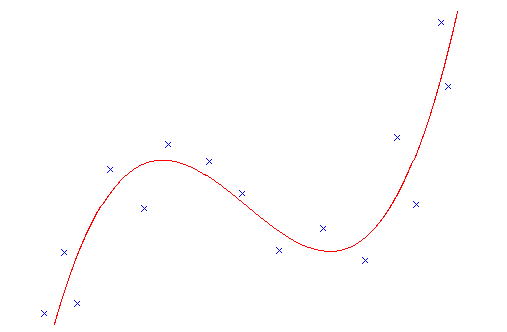
\includegraphics[keepaspectratio]{mathematica/cubica}
    \caption{Funzione cubica per l'interpolazione dei campioni di un processo\label{fig:andamentocubido}}
  \end{figure}

  \[ y=a_0 + a_1x+a_2x^2+a_3x^3 \]
Da qui, gli elementi del nostro modello saranno:

  \[
    Y=\begin{bmatrix} y_1\\y_2\\ \vdots \\ y_N \end{bmatrix}\quad
    u=\begin{bmatrix} x_1 \\ x_2 \\ \vdots \\ x_n \end{bmatrix}=\begin{bmatrix} u_1 \\ u_2 \\ \vdots \\u_n \end{bmatrix}\quad
    \theta=\begin{bmatrix} a_0 \\ a_1 \\ a_2 \\ a_3 \end{bmatrix}=\begin{bmatrix} \theta_1 \\ \theta_2 \\ \theta_3 \\ \theta_4 \end{bmatrix}
  \]
  
e quindi il modello:

  \[ \Phi(u,\theta)=\begin{bmatrix} \theta_1 + \theta_2u_1+\theta_3u_1^2+\theta_4u_1^3  \\ \vdots \\ \theta_1 + \theta_2u_N+\theta_3u_N^2+\theta_4u_N^3 \end{bmatrix} =\begin{bmatrix} 1 \ u_1 & u_1^2 & u_1^3 \\ & \vdots &    \\  1\ u_N & u_N^2 & u_N^3 \end{bmatrix}\cdot \begin{bmatrix} \theta_1 \\ \theta_2 \\ \theta_3 \\ \theta_4 \end{bmatrix} = \Phi(u) \cdot \theta \]
  
L'ultimo passaggio abbiamo potuto farlo perché il modello è lineare nei parametri, altrimenti, come nell'esempio precedente, non avremmo potuto ottenere questa semplificazione. La matrice $\Phi(u)$ che abbiamo ottenuto è detta matrice di sensitività \index{Matrice di sensistività} ed è costituita da tante colonne quanti sono i parametri e tante righe quante le osservazioni disponibili.
\end{esempio}

\begin{esempio} % ###########
Supponiamo di disporre di $q$ variabili e di voler spiegare $Y$ in funzione delle variabili; la prima approssimazione che si può fare è di tipo lineare e dire quindi che $Y$ è generata per combinazione lineare delle variabili di cui disponiamo. Questa forzatura alla linearità della funzione è detta regressione lineare \index{Regressione lineare}. Ovviamente non è detto che questa approssimazione sia esatta o sia la migliore, ma sicuramente è la più semplice da trattare e quindi preferibile quando possibile. La regressione lineare possiamo rappresentarla come combinazione lineare e quindi:

  \[ y(t)=\sum_{i=1}^{N} {\theta_i \cdot u_i(t)} \]
  
Nella rappresentazione come modello:

  \[ Y=\Phi(u,\theta)=\Phi(u) \cdot \theta \]
\end{esempio}

Dopo questa serie di esempi è evidente che il nostro scopo è quello di stimare il vettore dei parametri , dato che sono noti, rispettivamente sono i risultati e le variabili note a priori dal campione.

  %criteri di stima
  \section{Criteri di stima}
% ######################################################################## Stima ai mimimi quadrati - last square - LS
\subsection{Stima ai mimimi quadrati - last square - LS}
\index{Stima ai minimi quadrati (LS)}
Innanzi tutto, un'importante premessa è che il numero delle osservazioni $N$ sia almeno pari al numero dei parametri $q$ da stimare, quindi deve valere $N\geq q$. Nel caso in cui $N>q$, allora non sarà possibile trovare un modello che spieghi esattamente i dati per via degli errori di misura, inoltre, la realtà non è mai perfettamente modellabile. Per chiarire questo concetto di seguito vengono presentati due grafici che rappresentano i due casi $N=q$ e $N>q$:
% GRAFICI DEI DUE CASI
\textbf{GRAFICO DA FARE, NON VIENE BELLO}
\begin{figure}[htbp]
  \centering
  %\subfigure[Il rango non è massimo, ci sono infiniti punti di minimo\label{fig:grafo3Dnomin}]{\includegraphics[keepaspectratio]{mathematica/intercaso1}}
  
  %\subfigure[Il rango è massimo e il punto di minimo è unico\label{fig:grafo3Dmin}]{\includegraphics[keepaspectratio]{mathematica/intercaso2}}
  
  \caption{Confronto fra modelli che hanno tanti parametri quanti i dati, e modelli che hanno un numero di dati maggiore al numero di parametri.\label{fig:confrontomodellidatiparametri}}
\end{figure}

Come si può vedere, nel caso $N>q$ abbiamo dovuto usare una retta di regressione che minimizzasse gli errori, ma non ci è possibile creare una retta che passi per tutti i punti. Dato che il caso $N>q$ è la norma, e quindi non ci è possibile creare modelli esatti, ci "accontentiamo" che i residui\index{Residuo} \footnote{il residuo è l'errore commesso dal modello rispetto ad un particolare dato} siano piccoli $\varepsilon$ sia piccolo:

  \[ \varepsilon :=Y-\Phi(u)\cdot \theta \]
  
A esempio, potremmo desiderare che la somma dei quadrati dei residui sia piccola -SSR\footnote{Sum of Square Residual}- \index{Somma dei quadrati dei residui, Sum of Square Residual (SSR)} sia piccola:

  \[ SSR=\sum_{i=1}^{N}{\varepsilon_i^2 } = {||\varepsilon ||}^2 = (Y-\Phi(u)\cdot \theta)^T \cdot (Y-\Phi(u)\cdot \theta) \]
  
D'ora in avanti, per brevità, $\Phi\equiv \Phi(u)$. Il nostro interesse ora è trovare i parametri $\theta$ che minimizzino l'errore quadratico.
\paragraph{Teorema} supponendo che $rank[\Phi]=q$\footnote{ovvero che il rango della matrice di sensitività $\Phi$ sia pari a $q$, quindi che il numero di colonne linearmente indipendenti di $\Phi$ sia pari al numero di variabili $q$}, allora $ J(\theta):={||\varepsilon ||}^2 $ ha un minimo globale in corrispondenza di:
  \[ \theta=(\Phi^T\Phi)^{-1}\cdot \Phi^TY \]
Prima di procedere alla dimostrazione di questo teorema, si veda l'appendice \ref{app:operatorimatriciali}


\begin{dimostrazione}

  \[ rank[\Phi]=q \Longrightarrow det(\Phi^T\Phi) \ne 0 \]
  
se, per assurdo, $det(\Phi^T\Phi)=0$

  \[ 
    \begin{split}
      \exists x \ne 0 | \Phi^T\Phi x=0 &\Longrightarrow x^T\Phi^T\Phi x=0 \Longrightarrow ((\Phi x)^T\Phi x)=\| \Phi x \|^2 =0 \Longrightarrow \Phi x =0\\
       &\Longrightarrow rank[\Phi]<q \Longrightarrow \text{assurdo!} \Longrightarrow \exists (\Phi^T\Phi)^{-1} 
    \end{split} 
  \]
  
Ora che abbiamo verificato l'esistenza della matrice inversa, calcoliamo il gradiente dell'errore per cercare di minimizzarlo.

  \begin{gather*}
    J(\theta)=\varepsilon^T\varepsilon=(Y-\Phi\theta)^T(Y-\Phi\theta)\\
    \frac{dJ(\theta)}{d\theta}=2(Y-\Phi\theta)^T\Phi
  \end{gather*}
  
Vogliamo che $J(\theta)$ sia minimo per cui calcoliamo il valore del vettore $\theta$ che annulla il gradiente:

  \[ 
    \begin{split}\frac{dJ(\theta)}{d\theta} = 0 &\Leftrightarrow  2(Y-\Phi\theta)^T\Phi=Y^T-\theta^T\Phi^T=0 \Leftrightarrow Y^T\Phi=\theta^T\Phi^T\Phi \\ &\Leftrightarrow \Phi^TY=\Phi^T\Phi\theta \Leftrightarrow \theta= (\Phi^T\Phi)^{-1}\Phi^TY 
    \end{split}
  \]
  
Quello che abbiamo calcolato è un punto di massimo o minimo, per cui ora verifichiamo che sia di minimo calcolando la sua derivata seconda, se risulterà maggiore di zero allora sarà un minimo.

  \[ 
    \begin{split} \frac{d^2J(\theta)}{d\theta^2}&=\frac{d}{d\theta}\{\frac{dJ(\theta)}{d\theta}\}= \frac{d}{d\theta}\{2(Y-\Phi\theta)^T\Phi\}=2\frac{d}{d\theta}\{(Y-\Phi\theta)^T\}\Phi\\
  &=2\frac{d}{d\theta}\{Y^T-\theta^T\Phi^T\}\Phi=2\Phi^T\Phi 
    \end{split} 
  \] 
  
%FIXME che fine fa il - nella formula?
\begin{center}[FIXME: che fine fa il meno nella formula? Penso sia dovuto al penultimo passaggio, applicando T forse doveva andare via]\end{center}

Essendo il risultato una diade:

  \[ D=\Phi^T\Phi \geq 0 \Longrightarrow \frac{d^2J(\theta)}{d\theta^2}=2D \geq 0 \]
  
Come volevasi dimostrare, è un punto di minimo
\end{dimostrazione}

Possiamo quindi concludere che la stima LS è definita come:

  \[ \theta^{LS}=\arg \min_{\theta} J(\theta) \]
  
che, come abbiamo dimostrato, corrisponde a:

  \[ \theta^{LS}=(\Phi^T\Phi)^{-1}\Phi^TY \]

Il teorema appena dimostrato può anche essere interpretato geometricamente. Prendiamo il caso di soli due parametri e quindi $q=2$

\begin{figure}[htbp]
  \centering
  \subfigure[Il rango non è massimo, ci sono infiniti punti di minimo\label{fig:grafo3Dnomin}]{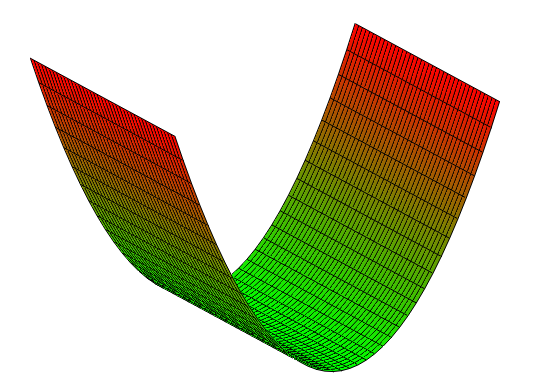
\includegraphics[scale=0.30]{img/graf3D1.png}}
  \subfigure[Il rango è massimo e il punto di minimo è unico\label{fig:grafo3Dmin}]{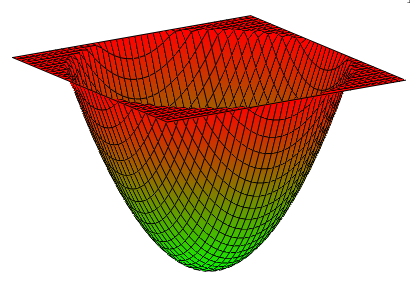
\includegraphics[scale=0.35]{img/graf3D2.png}}
  \caption{Identificabilità della soluzione\label{fig:identificabilitasoluzione}}
\end{figure}


Dati i grafici in figura \ref{fig:identificabilitasoluzione} vediamo nel grafico in figura \ref{fig:grafo3Dnomin} l'esempio in cui non si ha il rango massimo, infatti esistono infiniti punti di minimo. Nel grafico in figura \ref{fig:grafo3Dmin}, invece, abbiamo rango massimo ed un solo punto di minimo, quindi la soluzione si trova nel punto di minimo.\newline
Il problema studiato sin ora, ha fatto uso della supposizione che $rank[\Phi]=q\Rightarrow det(\Phi^T\Phi)\ne 0$, ma se così non fosse, abbiamo appena visto che si pone un problema di identificabilità\index{identificabilità}, ovvero, la soluzione non è unica come in figura \ref{fig:grafo3Dnomin}. Come scegliere la soluzione fra le infinite possibili? Supponiamo $q=3$ e che $rank[\Phi]=2$, quindi $rank[\Phi]<q$:

  \begin{gather*}
    \theta = \begin{bmatrix} \theta_1 \\ \theta_2 \\ \theta_3 \end{bmatrix}\quad
    \Phi=\begin{bmatrix} u_1(1) & u_2(1) & u_3(1) \\ u_1(2) & u_2(2) & u_3(2) \\ \vdots & \vdots & \vdots \\ u_1(N) &u_2(N) & u_3(N) \end{bmatrix}\\
    y(i)=\theta_1u_1(i)+\theta_2u_2(i)+\theta_3u_3(i)
  \end{gather*}
  
dato che $rank[\Phi]=2$, allora sappiamo che una colonna di $\Phi$ è linearmente dipendente dalle altre. Supponendo che la colonna dipendente sia quella associata a $u_3$ potremmo scriverla come:
  \[ u_3(i)=au_1(i)+bu_2(i) \]
dove i coefficienti $a$ e $b$ sono noti. Da qui possiamo scrivere:
  \[ y(i)=\theta_1u_1(i)+\theta_2u_2(i)+\theta_3(au_1(i)+bu_2(i)) = u_1(i)(\theta_1+a\theta_3)+u_2(i)(\theta_2+b\theta_3) \]
con questa riscrittura la variabile $u_3$ risulta inutile, potremmo quindi ridurre le matrici a:

    \[
      \bar{\theta} = \begin{bmatrix} \bar{\theta}_1 \\ \bar{\theta}_2 \end{bmatrix}= \begin{bmatrix}\theta_1+a\theta_3 \\ \theta_2+b\theta_3 \end{bmatrix} \quad
      \Phi=\begin{bmatrix} u_1(1) & u_2(1)  \\ u_1(2) & u_2(2)  \\ \vdots & \vdots  \\ u_1(N) &u_2(N) ) \end{bmatrix}
    \]
    
Risolvendo il modello per $\bar{\theta}$ ci siamo riportati nel caso $rank[\Phi]=q$ e quindi possiamo risolverlo come visto in precedenza ed avremo una soluzione unica data da:

  \[ \bar{\theta}^{LS}=\begin{bmatrix} \bar{\theta}_1^{LS} \\ \bar{\theta}_2^{LS} \end{bmatrix}=(\Phi^T\Phi)^{-1}\cdot \Phi^TY \]
  
Quali sono i casi in cui può capitare di avere $rank[\Phi]<q$?

  \begin{itemize}
    \item ingressi fissati
    \begin{itemize}
      \item modello sovraparametrizzato rispetto al fenomeno da descrivere; ad esempio l'uso di due variabili indipendenti ma con lo stesso effetto sulla variabile dipendente
      \item modello sovraparametrizzato rispetto all'informazione contenuta nei dati; ad esempio variabili dipendenti da altre
    \end{itemize}
    \item ingressi manipolabili
    \begin{itemize}
      \item se si usano più variabili per rendere più ricco di informazioni il modello
    \end{itemize}
  \end{itemize}
  
% ######################################################################## Stima ML
\subsection{Stima ML}
\index{Stima ML}
Per poter usare questo stimatore, occorre fare delle ipotesi sulla ddp dell'errore di misura. L'ipotesi fatta è che l'errore di misura $V$ abbia un andamento di tipo gaussiano:

  \[ V:=Y-\Phi\cdot\theta\quad
    V=\begin{bmatrix} V_1 \\ \vdots \\ V_N  \end{bmatrix}\quad
    V\sim N(0,\Sigma_V) , \Sigma_V>0 
  \]
  
Sotto l'ipotesi appena enunciata, con $rank[\Phi]=q$, se, inoltre, gli errori hanno tutti la stessa varianza $\Sigma_V=\sigma^2I$, allora valgono:

  \begin{align*}
    J^{ML}(\theta)&=\varepsilon ^T \Sigma_V^{-1}\varepsilon = \sum_{i=1}^{N}{\frac{\varepsilon_i^2}{\sigma_i^2} }\\
    \theta^{ML}&= \arg \max_{\theta} J^{ML}(\theta)=(\Phi^T\Sigma_V^{-1}\Phi)^{-1}\Phi^T\Sigma_V^{-1}Y=C \cdot Y\\
    E[{\theta^{ML}}]&=\theta \\
    Var[\theta^{ML}]&=(\Phi^T\Sigma_V^{-1}\Phi)^{-1}
  \end{align*}
  

\begin{dimostrazione} %###########
Dimostriamo la non polarizzazione dello stimatore:

  \[ E[\theta^{ML}]=E[CY]=C\cdot E[Y]=C\cdot E[\Phi\theta+V]=C\cdot E[\Phi\theta]+C\cdot E[V] \]
  
Sotto le ipotesi enunciate $E[V]=0$, quindi:

  \[ C\cdot E[\Phi\theta]+C\cdot E[V]=C\cdot E[\Phi\theta]=E[C\Phi\theta]=E\left[(\Phi^T\Sigma_V^{-1}\Phi)^{-1}\Phi^T\Sigma_V^{-1}\Phi\cdot\theta \right] \]
  
dato che $A^{-1}\cdot A=I$, ne consegue:

  \[ E\left[(\Phi^T\Sigma_V^{-1}\Phi)^{-1}\Phi^T\Sigma_V^{-1}\Phi\cdot\theta \right]=E[I\theta]=\theta \]
\end{dimostrazione}
\begin{dimostrazione} % ###########
Dimostriamo il risultato della varianza:
  \[ Var[\theta^{ML}]=Var[CY]=C\cdot Var[Y]\cdot C^T = C\cdot Var[\Phi\theta+V]\cdot C^T \]
dato che $\Phi\theta$ non è una V.C., non concorre a determinare la varianza, quindi:

  \[ 
  \begin{split}
      C\cdot Var[\Phi\theta+V]\cdot C^T&=C\cdot Var[V]\cdot C^T=C\Sigma_VC^T\\
      &=(\Phi^T\Sigma_V^{-1}\Phi)^{-1}\Phi^T\Sigma_V^{-1}\Sigma_V \Sigma_V^{-1} \Phi(\Phi^T\Sigma_V^{-1}\Phi)^{-1}\\
      &=(\Phi^T\Sigma_V^{-1}\Phi)^{-1}\Phi^T \Sigma_V^{-1} \Phi(\Phi^T\Sigma_V^{-1}\Phi)^{-1}\\
      &=(\Phi^T\Sigma_V^{-1}\Phi)^{-1}(\Phi^T \Sigma_V^{-1} \Phi)(\Phi^T\Sigma_V^{-1}\Phi)^{-1}=(\Phi^T\Sigma_V^{-1}\Phi)^{-1}
  \end{split} 
  \]
\end{dimostrazione}

Se, invece, sempre sotto l'ipotesi enunciata con $rank[\Phi]=q$, non avessimo la stessa varianza sugli errori, ma avessimo $\Sigma_V=\sigma^2\psi$, con $\sigma^2$ scalare incognito e $\psi$ matrice nota, allora:

  \begin{align*}
    \theta^{ML}&=(\Phi^T\frac{1}{\sigma^2}\psi^{-1}\Phi)^{-1}\Phi^T\frac{1}{\sigma^2}\psi^{-1}Y  =(\Phi^T\psi^{-1}\Phi)^{-1}\Phi^T\psi^{-1}Y  \\
    (\sigma^2)^{ML}&=\frac{1}{N}\{ (Y-\Phi\theta^{ML})^T\psi^{-1}(Y-\Phi\theta^{ML})\}=\frac{J_\psi^{ML}(\theta^{ML})}{N}\\
    J_\psi^{ML}&=\varepsilon ^T(\theta)\psi^{-1}\varepsilon (\theta)
  \end{align*} % nell'ultima formula non dovrebbe esserci anche \frac{1}{\sigma^2}
Da notare che $(\sigma^2)^{ML}$ è polarizzato e quindi per avere una stima non polarizzata bisogna usare:

  \[ (\sigma^2)^{ML}=\frac{J_\psi^{ML}(\theta^{ML})}{N-q} \]
  
\paragraph{Osservazione} La stima ML è meno sensibile alla presenza degli outlier rispetto alla stima MS come mostrato in figura \ref{fig:MLMSoutlier}

\begin{figure}[htbp]
  \centering
  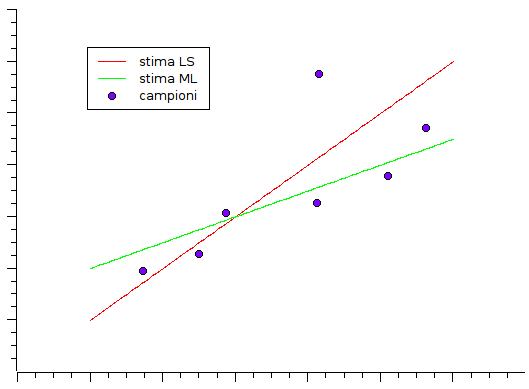
\includegraphics[scale=0.5]{img/outlier.png}
  \caption{Sensibilità delle stime ML e MS in presenza di outlier\label{fig:MLMSoutlier}}
\end{figure}

% ######################################################################## Intervalli di confidenza
\subsection{Intervalli di confidenza}
\index{Intervallo di confidenza}
Come già detto, fornire una stima senza dare informazioni sulla sua precisione è poco indicativo, vediamo quindi come calcolare l'intervallo di confidenza per la stima ML. Come visto dallo studio della stima ML ci son due casi: il primo dove l'errore di misura ha sempre la stessa varianza, quindi $\Sigma_V$ è una matrice nota; il secondo quando $\Sigma_V$ non è completamente nota ($\sigma^2$ è uno scalare sconosciuto e $\psi$ è una matrice nota).
Nel primo caso:

\begin{gather*}
    \theta^{ML}\sim N(\theta,\Sigma_{\theta^{ML}})\\
    I_\gamma(\theta_i)=\left[ \theta_i^{ML} - z_0\cdot\sigma_{\theta_i^{ML}}  ,  \theta_i^{ML} + z_0\cdot\sigma_{\theta_i^{ML}}\right]\quad \text{dove} \quad \sigma_{\theta_i^{ML}}^2 = \left[ \Sigma_{\theta^{ML}}\right]_{ii}\\
    z_0 | P(\left| Z \right| \leq z_0 ) =\gamma
\end{gather*}

nel secondo caso:

\begin{gather*}
  \Sigma_{\theta^{ML}}=\sigma^2(\Phi^T\psi^{-1}\Phi)^{-1}\\
  \frac{\theta_i^{ML}-\theta_i}{\hat{\sigma}_{\theta_i^{ML}}} \sim T_{N-q}\quad\text{dove}\quad\sigma_{\theta_i^{ML}}^2 = \left[ \Sigma_{\theta^{ML}}\right]_{ii}\\
  I_\gamma(\theta_i)=\left[ \theta_i^{ML} - t_0\cdot\sigma_{\theta_i^{ML}}  ,  \theta_i^{ML} + t_0\cdot\sigma_{\theta_i^{ML}}\right]\\
  t_0 | P(\left| T_{N-q} \right| \leq t_0 ) =\gamma
\end{gather*}


\begin{esempio}
Applichiamo la regressione lineare. Supponiamo di avere:

  \[ y(t)=\theta_1u_1(t)+ \dots +\theta_qu_q(t)+v(t) \]

Se la distribuzione dell'errore è di tipo gaussiano, allora la stima ML coincide con la stima LS e quindi $\Sigma_V=I$. Nel modello riconosciamo le seguenti matrici:

  \[ \Phi(u)\begin{bmatrix} u_1(1) & u_2(1) & \dots & u_q(1) \\ u_1(2) & u_2(2) & \dots & u_q(2)\\ \vdots & \vdots & \dots & \vdots \\ u_1(N) & u_2(N) & \dots & u_q(N) \end{bmatrix}=\begin{bmatrix} \varphi(1)^T \\  \varphi(2)^T \\ \vdots \\ \varphi(N)^T \end{bmatrix} \]

dove con $\varphi$ viene indicato il vettore di regressione. Dato che nel caso gaussiano i due metodi di stima sono uguali:
\begin{center}
  $\theta^{ML}=\theta^{LS}=(\Phi^t\Phi)^{-1}\Phi^TY=\sum_{i=1}^{N} \varphi(i) y(i)$
\end{center}
Se è soddisfatta la condizione di identificabilità $rank[\Phi]=q$
\begin{center}
  $(\sigma^2)^{ML}=\frac{J(\theta^{ML})}{N-q}=\frac{\sum_{i=1}^{N} \varepsilon^2(t) }{N-q}=\frac{\sum_{i=1}^{N} {\left(y(i)-\varphi(i)^T\theta^{ML}\right)^2}}{N-q}$\newline
  $\Sigma_{\theta^{ML}}=(\sigma^2)^{ML}(\Phi^T\Phi)^{-1}=(\sigma^2)^{ML} { (\varphi(i) \varphi^T(i) )^{-1}}$
\end{center}
Da qui il risultato finale:
\begin{center}
  $y(t)=\theta_1^{ML}u_1(t)+ \dots +\theta^{ML}_qu_q(t)+\varepsilon (t)$\newline
  $\varepsilon (t)=y(t)-\varphi^T(t)\theta^{ML}$
\end{center}
Da notare, in conclusione, che per ogni parametro stimato vi sarà una varianza associata da usarsi per la determinazione degli intervalli di confidenza.
\end{esempio}

  %scelta delle variabili
  \section{Scelta delle variabili}
In un modello in cui vi sono diverse variabili, ve ne potrebbero essere alcune che non influenzano il modello o comunque sono poco significative; il problema che ci poniamo ora è quello di individuare quali siano le variabili che influenzano poco o nulla il nostro modello.\newline
Per verificare se una variabile influenza il modello , si ragiona per assurdo assumendo che il parametro associato si a nullo.\newline
Volendo verificare se $\mu_k$ è utile al modello assumiamo, per assurdo che $\theta_k=0$ e verifichiamo se i dati sperimentali contraddicono l'assurdo.
  \begin{align*}
    \theta_k=0 \Rightarrow \frac{\theta_k^{ML}-E[\theta_k^{ML}]}{\sqrt{Var[\theta_k^{ML}]}}\sim Z\Rightarrow \frac{\theta_k^{ML}}{\sigma_k^{ML}}\sim Z
  \end{align*}
Nel 95\% dei casi vale:
  \[    \left| z \right| \leq 1.96 \Rightarrow \left| \frac{\theta_k^{ML}}{\sigma_k^{ML}} \right|\leq 1.96 \Rightarrow \left| \theta_k^{ML} \right| \leq 1.96\sigma_{\theta_k^{ML} }  \]
non abbiamo contraddetto l'assurdo e quindi è possibile che $\theta_k=0$ . Se, invece, vale:
  
    \[ |\theta_k^{ML} |>1.96\sigma_{\theta_k^{ML}} \]

allora siamo in una situazione che si verifica solo nel 5\% dei casi, ipotizzando $\theta_k=0$; quindi con buona probabilità diciamo che l'ipotesi è assurda e che $\theta_k\ne 0$ in modo significativo.\newline
In conclusione un metodo di scelta approssimativo della variabili è il seguente in tabella

  \begin{align*}
    | \theta_k^{ML} |&<2\sigma_{\theta_k^{ML}} \quad \text{non siamo sicuri sulla sua significatività della variabile}\\
    | \theta_k^{ML} |&>2\sigma_{\theta_k^{ML}} \quad \text{siamo certi che la variabile sia significativa}
  \end{align*}

Ovviamente , dato che non c'è certezza su $\theta_k=0$ se eliminiamo una variabile potremmo commettere degli errori.

  %validazione dei modelli
  \section{Validazione e scelta del modello}
Una volta creato il modello occorre chiedersi se quello prodotto è un buon modello e quali sono i suoi pregi e difetti rispetto ad altri. Quello che ci occorre ora sono dei metodi di validazione per i modelli con i quali possiamo mettere in atto dei confronti con altri. 
% ######################################################################## test del Chi Quadro
\subsection{Test del $\chi^2$}
\index{Test $\chi^2$}
Supponendo di avere a disposizione $N$ dati e di avere il modello:

    \[ Y=\Phi\cdot\theta^0+V, \quad Var[V]=\sigma^2\cdot I \]

come facciamo a dire se il modello li descrive adeguatamente? Supponiamo di fare una stima talmente precisa che:

    \[ \theta^{LS}\cong\theta^0 \Longrightarrow \varepsilon =Y-\Phi\cdot\theta^{LS}\cong V \]

e quindi la media dei residui del modello, "stima" l'errore di misura e quindi ci aspettiamo che:

    \[ \frac{1}{N}\sum_{i=1}^{N}{\varepsilon_i^2}\cong\sigma^2 \]

Allora se conosciamo $\sigma^2$ possiamo subito verificare che abbia lo stesso ordine di grandezza della varianza campionaria, e se differiscono in modo evidente, allora il modello spiega molto male i dati.
Ipotizziamo di aver "azzeccato" il modello vero, e che valga l'ipostesi che:

    \[ Y=\Phi\cdot\theta^0+V,  \quad  V\sim N(0,\sigma^2\cdot I) \]

ne consegue il seguente teorema.
\paragraph{Teorema} dividendo per $\sigma^2$ la somma dei quadrati dei residui\index{Somma dei quadrati dei residui, Sum of Square Residual (SSR)} -SSR- della stima LS, si ottiene una V.C. di tipo $\chi^2$ con $N-q$ gradi di libertà:
  \[ J=\frac{\varepsilon^T\varepsilon}{\sigma^2}\sim \chi^2(N-q) \]


L'idea è di usare il $\chi_{N-1}^2$ come riferimento sulla bontà di un modello e di verificare dove cade l'SSR rispetto al livello di significatività che vogliamo. 

\begin{figure}[htbp]
  \centering
  \includegraphics[keepaspectratio]{mathematica/chiquadrotest}
  \caption{test del Chi Quadro \label{fig:chiquadrotest}}
\end{figure}

Osservando la figura \ref{fig:chiquadrotest}, diciamo che scartiamo un modello se:

    \[ J>x_\alpha \]

mentre accettiamo il modello se:

    \[ J<x_\alpha \]

Ricordiamo che $J=\frac{\varepsilon^T\varepsilon}{\sigma^2}$ solo nel caso in cui $V\sim N(0,\Sigma_v)$, inoltre, il test si può estendere anche al caso in cui $V\sim N(0,\Sigma_V)$, avendo l'accortezza di usare $J=\varepsilon^T\Sigma_V\varepsilon$. \newline
Il test del $\chi^2$ ha due principali difetti:
\begin{itemize}
  \item non è facile capire la causa del fallimento: potrebbe effettivamente spiegare male il modello, oppure l'errore non è gaussiano, la varianza è errata per difetto, gli errori di misura hanno varianze diverse
  \item il test si basa sull'ipotesi che esista un vero modello lineare che spieghi i dati e che gli errori siano gaussiani. Queste due ipotesi sono molto semplificative perché la realtà è molto differente.
\end{itemize}
% ######################################################################## Test F
\subsection{Test F}
\index{Test F}
Supponiamo sempre di avere a che fare con modelli del tipo:

    \[ Y=\Phi\cdot\theta^0+V,  \quad  V\sim N(0,\sigma^2\cdot I) \]

Spesso non è evidente quale sia il modello migliore e vorremmo poter scegliere quello "ottimo". Prendiamo in considerazione i modelli matrioska\index{Modelli Matrioska}, ovvero sequenze di classi di modelli in cui per ogni classe sono comprese le precedenti come casi particolari. I polinomi, rappresentati in figura \ref{fig:matrioska}, sono un esempio di modelli matrioska.

\begin{figure}[htbp]
  \centering
  \includegraphics[keepaspectratio]{mathematica/matrioska}
  \caption{Plinomi: esempi di modelli matrioska\label{fig:matrioska}}
\end{figure}

In questo caso vediamo una rappresentazione tipica del problema: quale scelgo come modello? Come primo istinto si potrebbe pensare di usare il modello che minimizza l'SSR, ma sappiamo già che al crescere dell'ordine del modello l'SSR decresce e quindi l'SSR minimo è sempre in corrispondenza del modello di ordine maggiore e quindi più complesso. Ad esempio, per un campione di $N=100$ il modello migliore è approssimato da un polinomio di ordine $99$! Ovviamente non vi è alcun problema nell'usare polinomi di ordine elevato, con un altrettanto elevato numero di parametri, ma nella realtà i dati sono soggetti a rumore e quindi un polinomio di grado elevato viene influenzato dagli errori e quindi il modello seguirà troppo fedelmente l'andamento dei dati sperimentali e quindi dei suoi errori.\newline
Per evitare modelli complessi e sbagliati usiamo il principio di parsimonia, ovvero, usiamo la classe di ordine minore fintanto che la classe di ordine maggiore non ha un SSR molto minore. Perché il principio sia completo occorre indicare cosa s'intende per molto minore; usiamo come indica di riduzione percentuale dell'SSR:

    \[ f:=(N-k)\frac{SSR_{K-1}-SSR_k}{SSR_k} \]

$f$ è una V.C. distribuita come una $F$ di Fisher\index{Distribuzione di Fisher} con (1,N-k) gradi di libertà; inoltre osserviamo che:

    \[ \lim_{N-k\rightarrow\infty} {F(1,N-k)}=\chi_1^2 \]

A questo punto fissiamo il livello di significatività $\alpha$ e cerchiamo sulla tabella di Fischer:

    \[ f_\alpha \mid P(F(\,N-k)<f_\alpha)=1-\alpha \]

e quindi se $f>f_\alpha$ scelgo il modello $M_k$, altrimenti, se $f<f_\alpha$ scelgo il modello $M_{k-1}$
Concludiamo con alcune osservazioni sul test F. Non occorrono informazioni circa la varianza $\sigma^2$, inoltre il test è soggettivo, infatti, dobbiamo scegliere il parametro $\alpha$ con cui discriminare i modelli: con un $\alpha$ piccolo si tende a sottostimare l'ordine, mentre con un $\alpha$ grande si tende a sovrastimare l'ordine.\newline
Anche il test F è soggetto a difetti:
\begin{itemize}
  \item si applica solo a modelli matrioska
  \item dato che anche per il test F deve valere l'ipotesi di errori con andamento gaussiano vista per il $\chi^2$, il problema potrebbe essere che il modello vero non esista o non appartenga alla classe di modelli in esame.
\end{itemize}
% ######################################################################## Crossvalidazione
\subsection{Crossvalidazione}
\index{Test di crossvalidazione}
Quando si hanno a disposizione abbastanza dati possiamo dividerli in due gruppi: uno da usare per identificare il modello; l'altro per verificarlo ed eventualmente capire quale sia il migliore. Indichiamo con $Y^I$ l'insieme dei dati di identificazione del modello, mentre con $Y^V$ l'insieme dei dati di validazione del modello. Questo metodo di verifica è basato in tre passi:

\begin{enumerate}
  \item si considerano i vari modelli e si stimano i parametri usando l'insieme $Y^I$, ad esempio con la stima LS: $\theta^{LS}=(\Phi^T\Phi)^{-1}\Phi^TY^I$
  \item con i modelli identificati si cerca di prevedere i dati di validazione e si calcolano i residui, quindi: $SSR^V=\varepsilon^{V^T}\varepsilon^V$ dove $\varepsilon^V=Y-\hat{Y}$ e $\hat{Y}=\Phi^V\theta^{LS}$
  \item si sceglie il modello che genera l'$SSR^V$ minimo
\end{enumerate}

Facciamo alcune osservazioni sul metodo. 
\paragraph{Osservazione 1} Innanzitutto la divisione in due gruppi dev'essere casuale per evitare di influenzare il modello con scelte soggettive.
\paragraph{Osservazione 2} Quando si ha a che fare con dei modelli matrioska l'$SSR^I$ decresce al crescere dell'ordine, anche l'$SSR^V$ ha lo stesso comportamento, ma ad un certo punto il modello segue troppo fedelmente i dati di identificazione $Y^I$ e quindi l'$SSR^V$ riprende a crescere.
\paragraph{Osservazione 3} Talvolta questo processo suggerisce l'uso di modelli in cui alcuni parametri hanno una deviazione standard elevata. Conviene provare ad azzerarli e ricalcolare l'$SSR^V$. Se cambia di poco (1\%, 2\% ) rispetto al minimo, può essere conveniente usare il modello semplificato.
\paragraph{Osservazione 4} Non si cerca il modello vero, ma si cerca il migliore con una buona probabilità
% ######################################################################## Ordinary CrossValidation (OCV) e Generalized Cross Validation (GCV)
\subsection{Ordinary CrossValidation (OCV) e Generalized Cross Validation (GCV)}
\index{Test Ordinary CrossValidation (OCV)}
Nel caso in cui non si hanno a disposizione abbastanza dati per formare due gruppi, si può usare la OCV. Per identificare il modello e stimare i parametri si usano tutti i dati a disposizione meno uno, poi si calcola l'errore che si commette calcolando il valore scartato usando il modello. Si ripete questa procedura scartando man mano un elemento diverso l'indice OCV\footnote{altro non è che la media dei residui meno quello scartato}:

    \[ OCV=\frac{1}{N}\sum_{j=1}^{N}{\varepsilon_j^{(i)^2}},  \quad    {\varepsilon^{(i)}}=Y_i-\Phi^{(i)}\theta^{(i)^{LS}} \]

dove $Y_i$ è l'i-esimo valore scartato, $\Phi^{(i)}$ è il modello costruito senza l'i-esimo elemento e $\theta^{(i)^{LS}}$ è la stima dei parametri senza l'i-esimo elemento.\newline
Il grosso problema è che dobbiamo risolvere $N$ problemi di stima LS e questo è computazionalmente oneroso. Ci viene in aiuto il lemma del "lasciane uno fuori" (leaveout one lemma)

    \[ OCV=\frac{1}{N}\sum_{j=1}^{N}\frac{\varepsilon_j^2}{(1-H_{jj})^2}, \quad  H=\Phi(\Phi^T\Phi)^{-1}\Phi^T,  \quad  \varepsilon=Y-\Phi\theta^{LS} \]

In questo modo si stima una sola volta e si calcola la diagonale di $H$. Computazionalmente rimane più oneroso rispetto alla crossvalidazione; possiamo ridurre ulteriormente il carico con la Generalized Cross Validation\index{Test di Generalized CrossValidation (GCV)}:

    \[ GCV=\frac{1}{N}\frac{\sum_{j=1}^{N}{\varepsilon_j^2}}{(\frac{1}{N}Tr(1-H))^2}=\frac{1}{N}\frac{\sum_{j=1}^{N}{\varepsilon_j}}{(\frac{N-q}{N})^2}=SSR\frac{N}{(N-1)^2} \]

Il punto debole della crossvalidazione per i piccoli gruppi di dati sorge quando questi non hanno tutti la stessa varianza.
% ######################################################################## Final Prediction Error - FPE
\subsection{Final Prediction Error - FPE}
\index{Test Final Prediction Error (FPE)}
Se facessimo delle ipotesi sul meccanismo di generazione dei dati possiamo minimizzare $SSR^V$ senza calcolarla esplicitamente. Ipotizziamo\footnote{da notare che non stiamo ipotizzando la gaussianità dell'errore} che:

    \[ Y=\Phi\theta^0+V,\quad E[V]=0,\quad  Var[V]=\sigma^2 I \]

Supponendo ora di avere un vettore di parametri $\theta$ e che il modello per l'identificazione sia lo stesso della validazione, é dimostrabile che se si estrae un campione $Y^V$ di $N$ dati:

    \[ E[SSR^V]=N \sigma^2+(\theta-\theta^0)^T\Phi^T\Phi(\theta-\theta^0) \]

ovviamente $\theta=\theta^0$\footnote{$\theta=\theta^0$ significa che stiamo usando il modello vero} minimizza $E[SSR^V]$. Supponiamo ora che $\theta=\theta^{LS}$ sia la stima ottenuta da un campione $Y^I$, è dimostrabile che:

    \[ E[E[SSR^V]]=\sigma^2(N+q) \]

Da notare che vi è un valore atteso annidato perché abbiamo due estrazioni. Quello che abbiamo ricavato è una formulazione matematica del principio di parsimonia: se il modello vero è di ordine $k$, usare ordini superiori peggiora le prestazioni medie in fase di validazione. Molto spesso $\sigma^2$ non è nota; uno stimatore non polarizzato per $\sigma^2$ è:

    \[ \hat{\sigma}^2=\frac{SSR}{N-q} \]

Veniamo ora al criterio FPE vero e proprio. Tra diversi modelli matrioska con $q$ parametri fissati, si sceglie quello che minimizza la media stimata dell'$SSR^V$:

    \[ FPE=E[E[SSR^V]]=\hat{\sigma^2}(N+q)=\frac{N+q}{N-q}SSR \]

\paragraph{Osservazione 1} Al crescere di $q$ l'indice $FPE$ diminuisce con $SSR$, ma se $q$ cresce troppo, $FPE$ inizia a crescere, infatti $\lim_{q\rightarrow\infty}{\frac{N+q}{N-q}}=\infty$. Da questa osservazione concludiamo che esiste sempre un punto di minimo per l'indice $FPE$
\paragraph{Osservazione 2} Computazionalmente il criterio FPE è efficiente, infatti basta conoscere la stima dei parametri
\paragraph{Osservazione 3} Il criterio tende a sovrastimare (in media) l'ordine del modello al crescere dei dati. Non è uno stimatore consistente dell'ordine del modello,
% ######################################################################## Akaike Information Criterion - AIC
\subsection{Akaike Information Criterion - AIC}
\index{Test Akaike Information Criterion (AIC)}
Questo criterio vale sotto l'ipotesi di gaussianità dell'errore:

    \[ Y=\Phi\cdot\theta^0+V, \quad  V\sim N(0,\sigma^2\cdot I) \]

e che si stiano valutando dei modelli matrioska\index{Modelli matrioska}. Il criterio si basa sul calcolo della distanza fra la ddp dei dati e quella del modello stimato. Fra i modelli a $q$ parametri scelgo quello che minimizza:

    \[ AIC=\frac{2q}{N}+\ln SSR \]

\paragraph{Osservazione 1} $\lim_{N \rightarrow \infty} \ln FPE = AIC $ ne deduciamo che il criterio AIC tende a sovrastimare il modello al crescere dei dati
% ########################################################################
\subsection{Minimum Description Length - MDL}
\index{Test Minimum Description Length (MDL)}
Questo è un criterio che viene utilizzato quando si devono trasmettere dei dati. Invece di trasmettere i dati veri si può pensare di trasmettere la stima $\theta^{LS}$ e i residui $\varepsilon$ di modo che in ricezione si ricostruisca il dato con l'operazione:

    \[ Y=\Phi\theta^{LS}+\varepsilon \]

Il vantaggio è che se il modello è buono l'errore di predizione è piccolo e per codificarlo bastano pochi bit. Questo porta ad un risparmio in archiviazione e trasmissione.
Il criterio MDL serve a scegliere il modello con codifica più compatta. Sotto l'ipotesi:

    \[ Y=\Phi\cdot\theta^0+V, \quad V\sim N(0,\sigma^2\cdot I) \]

la scelta del modello si basa su quello che minimizza l'equazione:

    \[ MDL=\frac{\ln(N)+q}{N}+\ln(SSR) \]

\paragraph{Osservazione 1} Se l'ordine $q$ del modello aumenta, $SSR$ diminuisce e quindi anche il residuo $\varepsilon$; serviranno pochi bit a codificare $\varepsilon$ ma aumentano quelli necessari a codificare $\theta^{LS}$
\paragraph{Osservazione 2} Il criterio indica, asintotticamente al crescere dei dati, l'ordine vero del modello.
% ########################################################################
\subsection{Conclusioni}
Innanzi tutto dividiamo i criteri oggettivi da quello soggettivi. Indichiamo con criteri soggettivi quelli che necessitano di scelte soggettive come, ad esempio, il test F e il test $\chi^2$. Indichiamo con criteri oggettivi quelli basati sulla minimizazione di un indice di merito, come: crossvalidazione, OCV, GCV, FPE, AIC, MDL. La differenza è in realtà meno profonda di quanto sembri, infatti, per $N$ grande $FPE$ equivale al test F con $\alpha=0.157$, quindi FPE ha il 15.7\% di probabilità di scegliere (erroneamente) un modello più complesso.
L'unico metodo che non richiede ipotesi pesanti è la crossvalidazione, ma nella pratica FPE, AIC e MDL vengono usati senza particolari problemi.
Un suggerimento può essere quello di usare più di un criterio e valutare, inoltre, che la deviazione standard dei parametri non sia troppo discordante fra i diversi criteri.
In conclusione possiamo dire che, asintotticamente al crescere dei dati, il criterio MDL è meglio di FPE e AIC.

  %stimatore blue
  \section{Stimatore Blue Linear Unbiased Extimator - BLUE}
\index{Stima BLUE}
Se dalla stima ML togliamo l'ipotesi di gaussianità di $V$, ma assumiamo, genericamente:

    \[ Y=\Phi\theta+V, \quad  E[V]=0, \quad Var[V]=\sigma^2\psi \]

con $\psi$ noto e $\sigma^2$ eventualmente incognito.
\paragraph{Teorema Gauss-Markov}\index{Gauss-Markov, teorema} si consideri l'errore $J^M(\theta):=\varepsilon^T\psi^{-1}\varepsilon$ che è minimizzato da:

  \[ \theta^M=(\Phi^T\psi^{-1}\Phi)^{-1}\Phi^T\psi^{-1}Y \]
  
allora:
\begin{itemize}
  \item tra tutti gli stimatori lineari e non polarizzati, $\theta^M$ minimizza anche $Var[\hat{\theta}-\theta^0]$. Per questo motivo anche se non è il miglior stimatore in assoluto, è il migliore fra i lineari
  \item $Var[\theta^M]=\sigma^2(\Phi^T\psi^{-1}\Phi)^{-1}$
\end{itemize}
\paragraph{Osservazione 1} Non possiamo dire che è uno stimatore ML perché non ho le ipotesi sulla gaussianità dell'errore
\paragraph{Osservazione 2} Se $Var[V]=\sigma^2I$ allora $\theta^M=\theta^{LS}$
\paragraph{Osservazione 3} $\hat{\sigma}^2=\frac{J^M(\theta^M)}{N-q}$ è una stima non polarizzata
\paragraph{Osservazione 4} usando $\sigma^2$ o $\hat{\sigma}^2$ si può stimare $Var[\theta^M]=\Sigma_{\theta^M}=\hat{\sigma}^2(\Phi^T\psi^{-1}\Phi)^{-1}$
\paragraph{Osservazione 5} dato che non conosciamo la ddp di $V$ $J^M(\theta^M)$ non si comporta come una $\chi_{N-q}^2$. Inoltre non si può calcolare l'intervallo di confidenza $I_\gamma$; quello che possiamo fare però è fornire le deviazioni standard dei parametri.

  %stimatore di bayes
  \section{Stima di Bayes}
Essendo la stima di Bayes\index{Stima di Bayes} una stima a posteriori, abbiamo conoscenze a priori sui parametri $\theta$, quindi dobbiamo formulare nuove ipotesi:

  \begin{gather*}
     \exists \quad \text{un modello vero} \quad Y=\Phi\theta+V, \quad V\sim N(0,\Sigma_V) \\
     \Sigma_V>0,\quad \Theta\sim N(m_\Theta,\Sigma_\Theta),\quad \Sigma_\Theta>0,\quad  V,\Theta \quad \text{indipendenti} 
  \end{gather*}

\paragraph{Teorema} sotto le ipotesi appena citate, la stima di Bayes corrisponde a:
  \[ \theta^B=\arg \min_{\theta} \{ \varepsilon^T\Sigma_V^{-1} \varepsilon + (\theta-m_\Theta)^T\Sigma_\Theta^{-1}(\theta-m_\Theta)\} \]
che ha il suo punto di minimo in corrispondenza di:
  \[ \theta^B=(\Phi^T\Sigma_V^{-1}\Phi+\Sigma_\Theta^{-1})^{-1}(\Phi^T\Sigma_V^{-1}Y+\Sigma_\Theta^{-1}m_\Theta) \]
e la sua varianza corrisponde a:
  \[ Var[\theta^B]=(\Phi^T\Sigma_V^{-1}\Phi+\Sigma_\Theta^{-1})^{-1} \]
\paragraph{Osservazione 1} $\Sigma_\Theta^{-1} \rightarrow 0 $ allora $\theta^B \rightarrow \theta^{ML}$
\paragraph{Osservazione 2} non è necessario ipotizzare $rank[\Phi]=q$ perché sappiamo già che $\Sigma_\Theta>0$ e quindi $(\Phi^T\Sigma_V^{-1}\Phi+\Sigma_\Theta^{-1})^{-1}>0$ e quindi è invertibile
\paragraph{Osservazione 3} sfruttando informazioni a priori è possibile il caso $q>N$

  %stimatori non lineari nei parametri
  \section{Stima di modelli non lineari nei parametri}
Fin ora abbiamo visto solo come stimare con modelli lineari, quindi nel caso più semplice. Nel caso lineare ci troviamo nella forma:
  \[ Y=\Phi(u)\theta+V \]
ma nel caso non lineare nei parametri, il nostro sistema diventa:
  \[ Y=\Phi(u,\theta)+V \]
I criteri e le ipotesi degli stimatori visti precedentemente rimangono validi, la differenza fondamentale è che non è possibile trovare una forma esplicità dello stimatore (come abbiamo fatto e dimostrato nei casi lineari); ovvero non è possibile trovare un formula per il parametro che minimizza:
\[ J(\theta)=\varepsilon^T(\theta)\varepsilon \]
Per trovare un risultato si ricorre a metodi iterattivi. L'obiettivo degli algoritmi iterattivi è di partire da un punto ed avvicinarsi al minimo della funzione per passi.
\subsubsection{Algoritmo di Gauss -Newton}
\index{Gauss-Newton, algoritmo}
Supponiamo di voler risolvere:
\[ \hat{\theta}=\arg \min_{\theta} J(\theta)=\arg \min_{\theta} \varepsilon^T(\theta)\psi^{-1}\varepsilon(\theta)=\arg \min_{\theta} (Y-\Phi(u,\theta))^{-1}(Y-\Phi(u,\theta)) \]
(la presenza di $\psi$ è casuale, poteva non esserci, dipende dal problema). Definiamo ora con $\theta^k$ l'approssimazione di $\hat{\theta}$ al'iterazione k, e calcoliamo:

  \begin{align*}
    \Phi_\theta^k&={\frac{d\Phi(u,\theta)}{d\theta}}|_{\theta=\theta^k}\\
    \tilde{\theta}^k&=\theta-\theta^k\\
    \widetilde{Y}^k&=Y-\Phi(u,\theta^k) 
  \end{align*}
  
Per lo sviluppo di Taylor (troncata al primo grado) possiamo scrivere:

  \begin{gather*}
    \Phi(u,\theta) \cong \Phi(u,\theta^k) + \Phi_\theta^k(\theta-\theta^k)\\
    \varepsilon(\theta) = Y-\Phi(u,\theta) \cong Y-\Phi(u,\theta^k) - \Phi_\theta^k(\theta-\theta^k)=\widetilde{Y}^k-\Phi_\theta^k\tilde{\theta}^k
  \end{gather*}
  
Ne consegue quindi che:

  \[ J(\theta)\cong J^k(\tilde{\theta}^k)=(\widetilde{Y}^k-\Phi_\theta^k\tilde{\theta}^k)^T\psi^{-1}(\widetilde{Y}^k-\Phi_\theta^k\tilde{\theta}^k) \]
  
Ora la minimizzazione di $J^k(\tilde{\theta}^k)$ è un problema standard, infatti:

  \[ \hat{\tilde{\theta}}^k=((\Phi_\theta^k)^T\psi^{-1}\Phi_\theta^k)^{-1}(\Phi_\theta^k)^T\psi^{-1}\widetilde{Y}^k \]
  
ricordando che $\theta=\theta^k+\tilde{\theta}^k$, è logico che $\theta^{k+1}=\theta^k+\hat{\tilde{\theta}}^k$ e quindi:

  \[ \theta^{k+1}=\theta^k+[((\Phi_\theta^k)^T\psi^{-1}\Phi_\theta^k)^{-1}(\Phi_\theta^k)^T\psi^{-1}\widetilde{Y}^k] \]
  
\paragraph{Osservazione 1} Non c'è alcuna garanzia di convergenza ad una soluzione. Se anche dovesse convergere potrebbe finire in un minimo locale e non nel minimo globale che andiamo cercando. Eseguendo più volte l'algoritmo, se si ottengono valori diversi [FIXME: non si capisce cosa ci sia scritto negli appunti]
%FIXME NON SI CAPISCE COSA C'È SCRITTO NEGLI APPUNTI
\paragraph{Osservazione 2} Potrebbe accadere che $det(((\Phi_\theta^k)^T\psi^{-1}\Phi_\theta^k))\cong 0$ e quindi non è detto che il problema sia identificabile. Per ovviare a ciò si modifica l'algoritmo aggiungendo un parametro $\alpha^k$ che rende il determinante positivo:

  \[ \theta^{k+1}=\theta^k+[((\Phi_\theta^k)^T\psi^{-1}\Phi_\theta^k+\alpha_kI)^{-1}(\Phi_\theta^k)^T\psi^{-1}\widetilde{Y}^k] \]
  
Questa variazione va sotto il nome di Levenberg - Marquardt. La variabile $\alpha^k$ viene posta a zero quando il determinante è già significativamente diverso da zero, altrimenti viene posta ad un valore piccolo. In questo modo il determinante viene positivo e l'algoritmo prosegue nella minimizzazione
\paragraph{Osservazione 3} Convergenza quadratica nell'intorno del minimo:

  \[ \| \theta^{k+1}-\theta^k \|\leq \| \theta^k - \theta^{k-1}\|^2  \]
  
non garantisce la convergenza al minimo globale, quindi spesso si usano algoritmi medi.

\begin{center} \rule{300pt}{1pt} \end{center}
\begin{esempio} % ####################
Cinetica di un farmaco. Il problema è di capire quanto velocemente diminuisce la concentrazione $c(t)$ di farmaco presente nel corpo e quando ripetere la somministrazione:

\begin{figure}[htbp]
  \centering
  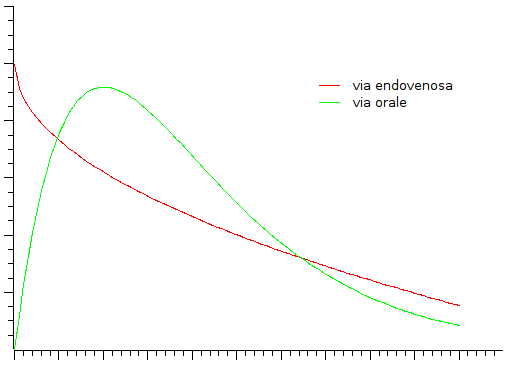
\includegraphics[scale=0.6]{img/cineticafarmaco.png}
  \caption{Cinetica di un farmaco\label{fig:cineticafarmaco}}
\end{figure}

%FIXME dagli appunti online è poco chiaro
[FIXME dagli appunti online è poco chiaro]
\end{esempio}

\begin{esempio} % ####################
Scelta tra due modelli
%FIXME dagli appunti online è poco chiaro
[FIXME dagli appunti online è poco chiaro]
\end{esempio}
\begin{center} \rule{300pt}{1pt} \end{center}


% PROCESSI CASUALI
\chapter{Processi casuali}
  \section{Processi casuali stazionari}
%FIXME non è chiaro
In generale è definito processo casuale\index{Processo casuale (PC)}\footnote{Può essere definito anche un segnale casuale} -PC- un esperimento casuale il cui esito è una funzione nel tempo $y(t)$. Questa funzione prende il nome di realizzazione. Nel corso di questa trattazione verranno considerati solo PC a tempo discreto rappresentati con un indice temporale intero.\newline
Un PC possiamo immaginarlo come un vettore di VC di lunghezza infinita, dove la posizione nel vettore corrisponde all'indice temporale, quindi per un tempo fissato $\bar{t}$, $y(\bar{t})$ corrisponde ad una singola VC. I PC che andiamo a considerare in questa trattazione sono quelli stazionari\index{Processo casuale stazionario}. Un PC si dice stazionario se per un qualsiasi numero $n$ di campioni scelti nel PC $t_1, ...t_n$, le proprietà statistiche non cambiano per un qualunque sfasamento temporale $\tau$ rispetto ai campioni originali\footnote{In altre parole le VC corrispondenti ad istanti diversi del processo casuale devono avere tutte la stessa ddp}.

\subsection{Media del primo ordine}
In generale $m_y(t)=E[y(t)]$ è una funzione del tempo $t$; occupandoci solo di processi stazionari, questo non è più vero, infatti, risulta $m_y(t)=m_y$. Se dipendesse dal tempo, violerebbe l'invarianza alle traslazioni temporali e quindi non può essere definito un PC stazionario.\newline
Per un PC stazionario è facile calcolare la $m_y$: basta calcolare la media campionaria del segnale $y(t)$.\newline 
A volte può essere utile studiare i PC stazionari con media nulla; possiamo ricondurre un qualsiasi PC stazionario a media non nulla in uno a media nulla. Considerando $\tilde{y}(t)=y(t)-m_y$ risulta che $E[\tilde{y}(t)]=0$; in questo modo ci siamo ricondatti ad un PC stazionario $\tilde{y}(t)$ a media nulla.\newline
%FIXME non mi è chiara l'ergodicità
Parliamo di processi ergodici\index{Ergodicità}... \textbf{[non mi è chiara l'ergodicità]}
\subsection{Covarianza ed autocovarianza}
Prima di introdurre la funzione di autocovarianza vediamo la funzione di covarianza, di cui l'autocovarianza è un caso particolare. La covarianza\index{Covarianza} $cov(X,Y)$ di due VC $X$,$Y$ è un indice di come le due VC variano assieme, in pratica è un indicatore di indipendenza; difatti se la covarianza è nulla $cov(X,Y)=0$ le due VC sono indipendenti. Il calcolo della covarianza è definito come:

  \[ cov(X,Y)=E\left[(X-E[X])(Y-E[Y])\right]=E[XY]-E[X]E[Y] \]
La covarianza gode delle seguenti proprietà:

  \begin{align*}
    cov(X,Y)&=cov(Y,X)\\
    cov(aX+b,Y)&=acov(X,Y)\\
    cov(X+Y,Z)&=cov(X,Z)+cov(Y,Z)
  \end{align*}

L'autocovarianza\index{Autocovarianza} è la covarianza su uno stesso segnale rispetto ad uno sfasamento temporale. Siano dati due istanti $t_1$,$t_2$ e il PC $x(t)$, definiamo l'autocovarianza come:
  \begin{align*}
    \gamma_{xx}(t_1,t_2)&=E\left[(x(t_1)-E[x(t_1)])(x(t_2)-E[x(t_2)])\right]\\
       \gamma_{xx}(\tau)&=E[(x(t)-E[x(t)])(x(t+\tau)-E[x(t)])] \quad \tau=t_1-t_2
  \end{align*}
Trattando PC stazionari, $E[x(t)]=m_x$ e quindi:

  \[ \gamma_{xx}(\tau)=E[(x(t)-m_x)(x(t+\tau)-m_x)] \]

\noindent L'autocovarianza ha le seguenti proprietà:

  \begin{align*}
    \gamma_{yy}(t_1,t_2)&=\gamma_{yy}(t_2,t_1)\\
          \gamma_{yy}(0)&=Var[y(t)]
  \end{align*}
        
% ########################################################################
% ########################################################################
\paragraph{Rumore Bianco - White Noise - WN}
Il rumore bianco\index{Rumore bianco}\index{White noise} è un particolare segnale che ha la caratteristica di essere totalmente incorrelato. Quindi $x(t)$ è $WN$ se $x(t_1)$ e $x(t_2)$ sono incorrelate $\forall \quad t_1\neq t_2$, ovvero: 

\[ \gamma_{xx}(t_1,t_2)=0 \quad t_1 \neq t_2 \Longrightarrow \text{PC stazionario}\quad \gamma_{xx}(\tau)=0 \quad r\neq 0 \]

\begin{figure}[htbp]
  \centering
  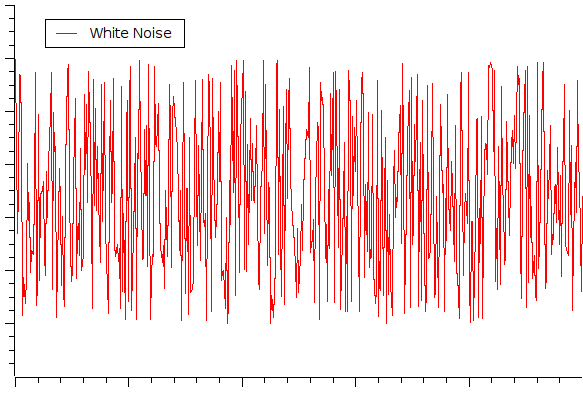
\includegraphics[scale=0.5]{img/whitenoise.png}
  \caption{Andamento del segnale white noise\label{fig:WN}}
\end{figure}

\noindent Un segnale di tipo WN, rappresentato in figura \ref{fig:WN}, viene indicato con:

\[x(t)\sim WN(m_x,\sigma_X^2) \]

Se due eventi $x(t_1)$ e $x(t_2)$ sono indipendenti si dice che $x(t)$ è un WN in senso stretto. Concludiamo con l'osservazione che un segnale WN è impredicibile, è il tipo di processo casuale più casuale che possa esistere, quindi è impossibile estrarre informazioni da un segnale di questo tipo.

  \section{Impariamo a leggere l'autocovarianza}
\begin{center}
[FIXME ci son molti grafici da disegnare, richiede molto tempo]
\end{center}
%FIXME TANTI GRAFICI
 %FIXME da fare
  \section{Trasformata Z}
La trasformata Z\citet{book:trasformataz}\index{Trasformata Z} permette di trasformare una funzione dal dominio del tempo discreto al dominio complesso discreto, ed è definita come segue:

\[ Z[x(i)]=X(z):=\sum_{i=-\infty}^{\infty}{x(i)\cdot z^{-i}},\quad z \in \mathbb{C}  \]

\noindent Vediamo due trasformate notevoli di cui faremo uso, ovvero, l'impulso (figura \ref{fig:impulsodiscreto}):

\[
x(i)=
\left\{
\begin{aligned}
1 \quad i=0 \\
0 \quad i\neq 0
\end{aligned}
\right.\Longrightarrow X(z)=1
\]

\begin{figure}[htbp]
  \centering
  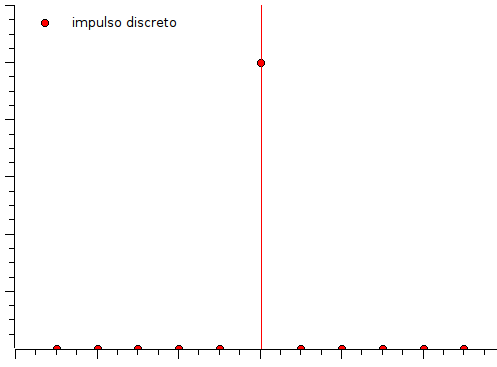
\includegraphics[scale=0.5]{img/impulsodiscreto.png}
  \caption{Impulso discreto\label{fig:impulsodiscreto}}
\end{figure}

\noindent e lo scalino (in figura \ref{fig:scalinodiscreto}):
\[
x(i)=
\left\{
\begin{aligned}
a \quad i\geq 0 \\
0 \quad i < 0
\end{aligned}
\right.\Longrightarrow X(z)=\frac{z}{z-a}
\]

\begin{figure}[htbp]
  \centering
  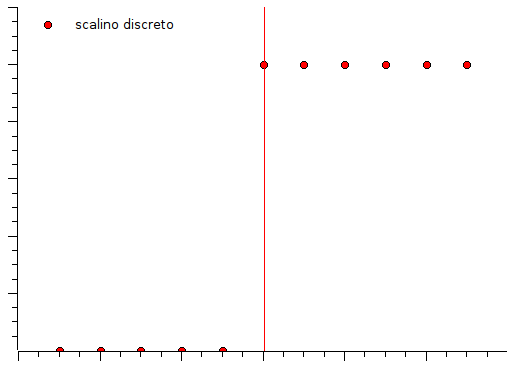
\includegraphics[scale=0.5]{img/scalinodiscreto.png}
  \caption{Scalino discreto\label{fig:scalinodiscreto}}
\end{figure}


La trasformata Z che consideriamo è sempre bilatera, ovvero esiste sia per posizioni negative che positive. Una funzione monolatera, di contro, esiste solo per i positivi.\newline
L'operazione di antitrasformazione è possibile ma è di uso poco pratico quindi non viene quasi mai utilizzata.
% ########################################################################
\subsection{Proprietà}
\paragraph{Proprietà 1 - Linearità} Se $x(i)$ e $y(i)$ sono due funzioni sugli interi con trasformata Zeta data rispettivamente da $X(z)$ e $Y(z)$, si ha che, qualunque siano le costanti $a$ e $b$:

  \[ Z[a\cdot x(i)+b\cdot y(i)]=a \cdot Z[x(i)] + b \cdot Z[y(i)]=aX(z)+bY(z) \]
  
con dominio che include o è uguale all'intersezione dei domini di $X(z)$ e $Y(z)$
\paragraph{Proprietà 2 - Traslazione} Se $x(i)$ è una funzione sugli interi con trasformata $X(z)$ e se $n_0 \in Z$ si ha:

  \[ Z[x(i-k)]=z^k\cdot Z[x(i)]=z^k\cdot X(z) \]
  
con dominio uguale al dominio di $X(z)$
\paragraph{Proprietà 3- Moltiplicazione per $i$} Se $x(i)$ è una funzione sugli interi con trasformata $X(z)$ allora:

  \[ Z[i \cdot x(i)]=-z\frac{dX(z)}{dz} \]
  
con dominio dato dalla stessa corona circolare di convergenza di $X(z)$
\paragraph{Proprietà 4 - Convoluzione} Se $x(i)$ e $y(i)$ sono due funzioni sugli interi con trasformata Zeta data rispettivamente da $X(z)$ e $Y(z)$ e se $x(i)$ e $y(i)$ hanno prodotto di convoluzione $x(i) \ast y(i) = \sum_{j=-\infty}^{\infty} {x(j)y(i-j)} = \sum_{j=-\infty}^{\infty} {x(i-j)y(j)}$, si ha che:

  \[ Z[x(i)\ast y(i)]=Z[x(i)]\ast Z[y(i)]=X(z)Y(z) \]
  
con dominio che include o è uguale all'intersezione dei domini di $x(z)$ e di $Y(z)$
% ########################################################################
\subsection{Confronto con Fourier}
Esiste una relazione fra la trasformata Z e la trasformata di Fourier\index{Trasformata di Fourier}. Sia $x(i)$ tale che $\sum_{i=-\infty}^{\infty} {|x(i)|}<\infty$\footnote{ovvero converge a zero velocemente}, allora esiste la trasformata di Fourier:

  \[ F[x(t)]=\sum_{t=-\infty}^{\infty}{x(t)e^{-j\omega t}}=\sum_{t=-\infty}^{\infty}{x(t)z^{-t}}, \quad j=\sqrt{-1},e^{j\omega}=z \]
  
\noindent e inoltre:

  \[ F(x(t))=X(e^{j\omega}) \]
  
%GRAFICHETTI
\paragraph{Osservazione 1} La trasformata Z è una funzione complessa di variabile complessa, mentre la trasformata di Fourier è una funzione complessa di variabile reale
\paragraph{Osservazione 2} L'antitrasformazione con la trasformata di Fourier è più semplice

  \section{Densità spettrale di potenza}
Sia $x(t)$ un processo casuale stazionario, definiamo la sua densità spettrale di potenza\index{Densità spettrale di potenza} come la trasformata di Fourier\index{Trasformata di Forurier} dell'autocovarianza\index{autocovarianza}:

  \[ \Gamma_{xx}(\omega)=F[\gamma_{xx}(t)]=\sum_{\tau=-\infty}^{\infty}{\gamma_{xx}(\tau)e^{-j\omega\tau}} \]
  
\noindent spesso si fa anche riferimento alla definizione che fa uso della trasformata Z\index{Trasformata Z} dell'autocovarianza:

  \[ \Phi_{xx}(Z)=Z[\gamma_{xx}(t)]= \sum_{\tau=-\infty}^{\infty}{\gamma_{xx}(\tau)z^{-\tau}} \]
  
\subsection{Proprietà}
\paragraph{Proprietà 1} $\Gamma_{xx}(\omega)$ è sempre reale, $\Gamma_{xx}(\omega) \in \mathbb{R} $
\paragraph{Proprietà 2} $\Gamma_{xx}(\omega)$ è sempre pari, $\Gamma_{xx}(-\omega)=\Gamma_{xx}(\omega)$
\paragraph{Proprietà 3} $\Gamma_{xx}(\omega)$ è sempre positiva
\paragraph{Proprietà 4} $\Gamma_{xx}(\omega)$ è sempre $2\pi$ periodica
%% grafichetto
\paragraph{Proprietà 4} $\Gamma_{xx}(\omega)$ ha sempre un'antitrasformata

  \[ \gamma(\tau)=\frac{1}{2\pi}\int_{-\pi}^{\pi}{\Gamma_{xx}(\omega)e^{j\omega\tau}d\omega} \]
  
ed inoltre, $\gamma_{xx}(0)=Var[x(t)]$, da qui possiamo calcolare l'integrale:

  \[  \int_{-\pi}^{\pi}{\Gamma_{xx}(\omega)e^{j\omega\tau}d\omega} = 2\pi Var[x(t)]\]
  
Da notare che un processo che sottende un'area grande significa che ha una varianza elevata.

  \section{Interpretazione dell'autocovarianza e della densità spettrale di potenza}
% TANTI GRAFICI
[tanti grafici da disegnare, ci vuole molto tempo]
 %FIXME da fare
  \section{Stima della l'autocoovarianza}
\index{Stima dell'autocovarianza}
Supponendo che $x(t)$ sia un PC stazionario ergodico, che abbia valore atteso nullo $E[x(t)]=0$ e che siano disponibili i dati $x(t) \quad t=0,...,N-1$, un possibile stimatore dell'autocoovarianza\index{Autocovarianza} è dato da:

  \[ c_{xx}^{'}(\tau)=\frac{1}{N-|\tau |}\sum_{i=0}^{N-|\tau |-1}{x(i)x(i+\tau )} \quad, |\tau |<N \]
  
\noindent dove con $\tau$ indichiamo lo spostamento rispetto al valore di riferimento.
\paragraph{Osservazione 1} Lo stimatore non è polarizzato, infatti $E[c_{xx}^{'}]=\gamma_{xx}(\tau)$

%FIXME
\begin{center}[FIXME DIMOSTRAZIONCINA CHE NON CAPISCO]\end{center}

\paragraph{Osservazione 2} Lo stimatore è consistente. Per $\tau$ fissato $\lim_{N\rightarrow\infty}{Var[c_{xx}^{'}(\tau )]}=0$, ovvero, al crescere dei dati tende ad una delta di Dirac.
%FIXME fare il grafico
\newline[GRAFICO TENDENZA]
\paragraph{Osservazione 3} Per $N$ fissato si vede che per $\tau\cong N$ la varianza $Var[c_{xx}^{'}]$ diventa grande, questo perché nel processo di stima vengono inseriti pochi termini $N-|\tau|-1$; se la varianza è grande siamo tentati a scartare il risultato.\newline\newline
Uno stimatore alternativo per la l'autocovarianza è il seguente:

  \[ c_{xx}^{'}(\tau)=\frac{1}{N}\sum_{i=0}^{N-|\tau |-1}{x(i)x(i+\tau )} \quad, |\tau |<N \]
  
\paragraph{Osservazione 1} Lo stimatore è polarizzato, ma è asintotticamente non polarizzato:

  \[ c_{xx}(\tau)=\frac{N-|\tau |}{N}c_{xx}^{'} \Longrightarrow E[c_{xx}(\tau )]=\frac{N-|\tau |}{N}\gamma_{xx}(\tau )\]
  
\paragraph{Osservazione 2} Lo stimatore è consistente. Per $\tau$ fissato $\lim_{N\rightarrow\infty}{Var[c_{xx}^{'}(\tau )]}=0$, ovvero, al crescere dei dati tende ad una delta di Dirac.
\paragraph{Osservazione 3} Per $N$ fissato e $\tau\cong N$, si ha che il valore atteso della stima $E[c_{xx}(\tau )]$ diminuisce al crescere di $\tau$, questo significa che peggiora la polarizzazione vicino ai bordi.\newline\newline
Per questi stimatori è possibile definire degli intervalli di confidenza ma sono troppo complicati da calcolare e sono strettamente dipendenti dal processo che si sta studiando.\newline

%FIXME
\begin{center}[FIXME, PERCHÉ? Chi è il soggetto? Copiato pari pari dagli appunti]\end{center}
\textit{In conclusione è meglio propendere per lo zero piuttosto che fornire numeri di cui non si conosce esattamente la natura. Inoltre, la maggior parte dei processi casuali stazionari è tale che $\lim_{|\tau|\rightarrow\infty}{\gamma_{xx}(\tau)}=0$. Per prudenza consideriamo $c_{xx}(\tau)$ sono per $|\tau|\leq \frac{N}{4}$}

  \section{Stima dello spettro - Periodogrammi}
L'idea di base nella stima dello spettro\index{Stima dello spettro} è di trasformare secondo Fourier\index{Trasformata di Forurier} la stima dell'autocoovarianza\index{Stima dell'autocovarianza} $c_{xx}$ invece che l'autocoovarianza\index{Autocovarianza} $\gamma_{xx}$. Otteniamo quindi il seguente periodogramma:

  \[ I_N(\omega):=\sum_{\tau=-(N-1)}^{N-1}{c_{xx}(\tau)e^{-j\omega\tau}} \]
  
Da notare che non eseguiamo la sommatoria in $[-\infty;\infty]$ perché stiamo usano $c_{xx}$ che è definita solo in $[-(N-1);N-1]$ e la consideriamo nulla altrove, quindi sarebbe uno spreco computazionale ampliare la sommatoria.

\subsection{Media di periodogrammi - Metodo di Bartlett}
Per processi che si comportano come il rumore bianco, il periodogramma non è un buon stimatore perché ha una varianza troppo elevata. Si cerca di compensare con la media dei periodogrammi\index{Media dei periodogrammi}. Per calcolare questo stimatore, si divide l'intervallo $[0,N-1]$ in intervalli di ampezza $M$, chiamati finestre, e per ognuno di questi si calcola la media del periodogramma\footnote{limitato all'intervalli di ampiezza $M$ che si sta considerando}. Con questo algoritmo riusciamo a ridurre la varianza di un fattore $\frac{M}{N}$
\paragraph{Osservazione 1} La polarizzazione è la stessa di $I_M(\omega)$
\paragraph{Osservazione 2} Per ridurre la varianza dobbiamo aumentare il numero di finestre $K=\frac{N}{M}$, ma questo significa avere finestre piccole che creano periodi peggiori.
\paragraph{Osservazione 3} Se siamo a conoscenza del fatto che nello spettro vi sono dei picchi sottile, allora dovremo scegliere l'ampiezza delle finestre $M$ abbastanza grande, di contro avendo finestre grandi la varianza viene ridotta di poco.\newline\newline
Dalle osservazioni 2 e 3 viene difficile scegliere con precisione l'ampiezza da usare per le finestre, l'unico metodo è procedere per tentativi e scegliere il caso migliore.


% SISTEMI DINAMICI
\chapter{Sistemi Dinamici}
  \section{Sistemi dinamici lineari invarianti a tempo discreto}
I sistemi\footnote{oggetto di studio di altri corsi, si consiglia eventualmente di ripassare questi argomenti} che andiamo a considerare godono delle seguenti proprietà:
\begin{itemize}
  \item sono lineari\footnote{gli effetti seguono linearmente le cause}
  \item sono invarianti\footnote{le caratteristiche del processo non variano nel tempo}
  \item sono a tempo discreto\footnote{osserviamo il comportamento ad intervalli regolari}
\end{itemize}
e per questo definiti Sistemi dinamici lineari invarianti a tempo discreto\index{Sistemi dinamici lineari invarianti a tempo discreto}
\begin{figure}[htbp]\Large
  \centering
  \[
    \begin{CD}
      u(t) @>>> \framebox{$S$} @>>> y(t)
    \end{CD}
  \]
  \caption{Sistema dinamico \label{fig:sistemadinamico}}
\end{figure}

\noindent Questi sistemi obbediscono alla seguente relazione\footnote{è la convoluzione discreta fra le cause $u()$ e la funzione di trasferimento $g()$}:

\[ y(t)=\sum_{i=-\infty}^{t}{g(t-i)u(i)}=\sum_{j=0}^{\infty}{g(j)u(t-j)}  \]

Misurando la risposta impulsiva del sistema, vediamo che questa corrisponde alla funzione di trasferimento\index{Funzione di trasferimento} $y(t)=g(t)$ dato che la convoluzione ha un solo termine non nullo in corrispondenza di $u(t)=1,\quad t=0$
\subsection{Funzione di trasferimento}
La funzione di trasferimento\index{Funzione di trasferimento} è una funzione che mette in relazione un segnale in ingresso con uno in uscita.

  \begin{figure}[htbp]\Large
    \centering
    \[
      \begin{CD}
        u(t) @>>> \framebox{$g(t)$} @>>> y(t)
      \end{CD}
    \]
    \caption{Funzione di trasferimento nel tempo \label{fig:funztrasftempo}}
  \end{figure}
  
Nel corso del nostro studio definiamo la funzione di traferimento nel dominio della trasformata Z\index{Trasformata Z}:

  \[ G(z)=Z[g(t)]=\sum_{t=0}^{\infty}{g(t)z^{-t}} \]

Come visto nei capitoli precedenti, operare nel dominio della trasformata Z ci permette di calcolare molto facilmente la convoluzione, infatti risulterà essere:

  \[ Y(z)=G(z)U(z)\]


  \begin{figure}[htbp]\Large
    \centering
    \[
      \begin{CD}
        U(z) @>>> \framebox{$G(z)$} @>>> Y(z)
      \end{CD}
    \]
    \caption{Funzione di trasferimento nel dominio Z \label{fig:funztrasfz}}
  \end{figure}
  

Un generico sistema $S$ viene considerato a dimensioni finite\index{Sistema a dimensioni finite}, se la relazione che lega le cause $u(t)$ agli effetti $y(t)$ è esprimibile mediante un'equazione alle differenze:

  \[ y(t)=\sum_{i=1}^{n_a} {a_iy(t-i)}+\sum_{i=0}^{n_b} {b_iu(t-i)} \]
  
Se abbiamo a che fare con un sistema a dimensioni finite, allora la funzione di trasferimento $G(z)$ è razionale fratta\index{Funzione di trasferimento razionale fratta}, ovvero una frazione fra polinomi:

  \[ G(z)=\frac{\sum_{i=0}^{n_b} {b_iz^{-i}}}{1-\sum_{i=1}^{n_a} {a_iz^{-i}}}=\frac{N_G(z)}{D_G(z)} \]

da cui possiamo ricavare gli zeri\footnote{tutti i termini che annullano il numeratore} e i poli\footnote{tutti i termini che annullano il denominatore} rispettivamente da $N_G$ e $D_G$. D'ora in avanti considereremo solo sistemi a dimensioni finite, quindi con funzioni di trasferimento razionali fratte.

\begin{esempio}
  \begin{align*}
    y(t)&=ay(t-1)+u(t)+bu(t-1)\\
    Y(z)&=az^{-1}Y(z)+U(z)+bz^{-1}U(z) \Longrightarrow (1-az^{-1})Y(z)=(1+bz^{-1})U(z) \\
    &\Longrightarrow Y(z)=\frac{1+bz^{-1}}{1-az^{-1}}U(z)=\frac{z+b}{z-a}U(z)=G(z)U(z)
  \end{align*}
\end{esempio}

\paragraph{Stabilità} Un generico sistema $S$ è definito stabile (asintotticamente) se:
  
  \[ \lim_{t\rightarrow\infty}{g(t)}=0 \]

Questo perché gli effetti dell'impulso si smorzano nel tempo. Nel caso di sitemi a dimensioni finite, essi sono stabili se e solo se $\|a\|<1$, ovvero tutti i poli sono, in modulo, inferiori ad 1.

\begin{esempio}
  \begin{align*}
    y(t)&=ay(t-1)+u(t)\\
    Y(z)&=az^{-1}Y(z)+U(z) \Longrightarrow G(z)=\frac{z}{z-a}\\
    &\text{polo in }z=a \Longrightarrow G(z) \text{ stabile} \Leftrightarrow \|a\|<1
  \end{align*}
\end{esempio}

\paragraph{Guadagno} Il guadagno di un sistema è definito come:
  
  \[ \mu=G(1)=\sum_{t=0}^{\infty}g(t) \]
  
Supponiamo di avere in ingresso una funzione a scalino unitario $u(t)=sca(t)$ ed un sistema stabile con guadagno finito; in uscita il risultato tenerà asintotticamente al valore del guadagno:

  \[ \lim_{t\rightarrow\infty}{y(t)}=\mu \]

\paragraph{Teorema della risposta in frequenza}\index{Risposta in frequenza} Si consideri un sistema asintotticamente stabile. Sia $u(t)=A\sin(\omega t)$, allora $\lim_{t\rightarrow\infty}{y(t)-\tilde{y}(t)}=0$, ovvero il sistema si stabilizza a $\tilde{y}(t)$, dove:

  \[ \tilde{y}(t)=A|G(e^{j\omega})|\sin(\omega t + \arg[G(e^{j\omega})]) \]
  
In altre parole, un ingresso sinosuidale $u(t)$ di pulsazione $\omega$ produce, asintotticamente, un'uscita $y(t)$ con la stessa pulsazione ma ampiezza e fase dipendenti dalla funzione di trasferimento in $G(z)=G(e^{j\omega})$. $G(e^{j\omega})$ è detta risposta in frequenza. Un metodo rapido per intuire la forma del suo modulo $|G(e^{j\omega})|$ è il metodo del "tendone da circo". In pratica, in una rappresentazione 3D, ovunque siano presenti dei poli il modulo della risposta in frequenza tende all'infinito, mentre è uguale a 0 in corrispondenza degli zeri. 
%FIXME
[FIXME fare i grafici per il tendone da circo]
[FIXME è consigliabile quindi preferire le regioni non troppo vicine ai poli, altrimenti il sistema entra in risonanza e vi è una risposta troppo alta, idealmente infinita]

  \section{Sistemi lineari (con ingressi) stocastici}
Un sistema lineare con ingresso stocastico\index{Sistema lineare con ingresso stocastico}, non è altro che un sistema con in ingresso un PC stazionario (in senso lato) $u(t)$ con momenti del primo e secondo ordine:

  \begin{align*}
    m_u&=E[U(t)] &\text{non dipendente da}\quad &t\\
    \gamma_{uu}&=Cov[u(t),u(t+\tau)] &\text{dipende solo da}\quad &\tau
  \end{align*} 
  
\begin{figure}[htbp]\Large
  \centering
  \[
    \begin{CD}
      u(t) @>>> \framebox{$G(z)$} @>>> y(t)
    \end{CD}
  \]
  \caption{Sistema dinamico \label{fig:sistlinstoc}}
\end{figure}

\noindent Inoltre consideriamo funzioni di straferimento $G(z)$ con poli stabili\footnote{in modulo minori di 1}. Da queste premesse ne consegue che:

  \[ m_y=E[y(t)]=G(1)m_u=\mu m_u \]

\paragraph{Teorema} Se $u(t)$ è un PC stazionario e il sistema è stabile, allora anche $y(t)$ è un PC stazionario; se così non fosse non potremmo parlare di spettro di $y(t)$

Da qui possiamo fare alcune considerazioni sulla densità spettrale di potenza\footnote{qui rappresentate sia nel dominio della trasformata Z sia nel dominio della trasformata di Fourier}\index{Densità spettrale di potenza} del segnale d'uscita $y(t)$, possiamo scrivere:

  \begin{align*}
    \Gamma_{yy}(\omega)&=|G(e^{j\omega})|^2\Gamma_{uu}(\omega)\\
    \Phi_{yy}(z)&=G(z)G(z^{-1})\Phi_{uu}(z)
  \end{align*}
  
\noindent estendibile al caso vettoriale:

  \begin{align*}
    \Gamma_{yy}(\omega)&=G(e^{j\omega})\Gamma_{uu}(\omega)G^T(e^{-j\omega})\\
    \Phi_{yy}(z)&=G(z)\Phi_{uu}(z)G^{-1}(z^{-1})
  \end{align*}

\paragraph{Osservazione 1} In pratica $|G(e^{j\omega})|$ è un "modulatore" della densità spettrale di ingresso.
\paragraph{Osservazione 2} Dato $\Phi_{yy}(z)$, se riusciamo a trovare $G(z)$ stabile e tale che $\Phi_{yy}=G(z)G(z^{-1})$, allora possiamo simulare\footnote{ovvero ottenere un segnale $y(t)$ desiderato} $y(t)$ come l'uscita di un sistema $G(z)$ con ingresso un segnale $w(t)\sim WN(0,1)$. Questo perché la densità spettrale di potenza del rumore bianco è unitaria su tutto lo spettro:

  \[ Y(z)=G(z)W(z) \Longrightarrow  \Phi_{yy}(z)=G(z)G(z^{-1})\Phi_{ww}(z)=G(z)G(z^{-1}) \]
  
In questo caso si parla di PC stazionari a spettro razionale. Da osservare che in un processo di questo tipo, se $\bar{z}$ è un polo/zero allora sono anche poli/zeri anche l'inverso e i rispettivi coniugati: $\frac{1}{\bar{z}},\bar{z}^{*},\frac{1}{\bar{z}^{*}}$

  \section{Processi Moving Average - MA}

\begin{figure}[htbp]\Large
  \centering
  \[
    \begin{CD}
      \begin{CD}
        w(t) @>>>\\
        w(t-1) @>>>\\
          ...  @>>>\\
        w(t-n) @>>>
      \end{CD}
      \framebox{$G(z)$} @>>> y(t)
    \end{CD}
  \]
  \caption{Sistema dinamico Moving Average \label{fig:ma}}
\end{figure}

\noindent Un processo di tipo Moving Average\index{Moving Average (MA)}, $MA(n)$ è definito come:

  \[ y(t)=\sum_{i=0}^{n}{c_iw(t-i)}, \quad w(t) \sim WN(0,\sigma^2) \]

\noindent con funzione di trasferimento:

  \[ G(z)=\sum_{i=0}^{n}{c_iz^{-i}}=\frac{1}{z^n}\sum_{i=0}^{n}{c_iz^{n-i}} \]



Notiamo che la funzione di traferimento ha $n$ poli nell'origine ed $n$ zeri; dato che i poli sono tutti nell'origine allora $G(z)$ è stabile e quindi $y(t)$ è un PC stazionario. Circa le proprietà statistiche, vediamo il valore atteso e l'autocovarianza:

  \begin{align*}
    E[y(t)]&=\sum_{i=0}^{n}{c_iE[w(t-i)]}\\
    \gamma_{yy}(\tau)&=E[y(t)y(t+\tau)]
  \end{align*}

Mentre il calcolo del valore atteso è di immediato risultato, quello dell'autocovarianza necessita una verifica per passi. Iniziamo col calcolare l'autocoovarianza per $\tau=0$, che corrisponde alla varianza, infatti:

  \[ 
    \begin{split}
  \gamma_{yy}(0)&=E[y(t)y(t)]=E[y^2(t)]=Var[y(t)]=\\
                &=Var[\sum_{i=0}^{n}{c_iw(t-i)}]=\sum_{i=0}^{n}{Var[c_iw(t-i)]}=\\
                &=\sum_{i=0}^{n}{c_i^2Var[w(t-i)]}=\sum_{i=0}^{n}{c_i^2\sigma^2}=\sigma^2\sum_{i=0}^{n}{c_i^2} 
    \end{split}
  \]
  
Dato che stiamo considerando PC stazionari, ovvero le proprietà statistiche non cambiano nel tempo, abbiamo semplificato l'equazione ponendo $Var[w(t-i)]=\sigma^2$. Passiamo ora a considerare $\tau=1$:
 
  \[ 
    \begin{split}
  \gamma_{yy}(1)&=E[y(t)y(t-1)]=E\left[ \left( \sum_{i=0}^{n}{c_iw(t-i)}\right)\left( \sum_{i=0}^{n}{c_iw(t-i+1)}\right)    \right]=\\
  &=E[(c_0w(t)+c_1w(t-1)+c_2w(t-2)+...+c_nw(t-n))\cdot\\
  &\cdot(c_0w(t+1)+c_1w(t)+c_2w(t-1)+...+c_nw(t-n+1))]=\\
  &=E[c_0c_0w(t)w(t+1)+c_0c_1w(t)w(t)+c_0c_2w(t)w(t-1)+...]=\\
  &=c_0c_1E[w(t)w(t+1)]+c_0c_1E[w(t)w(t)]+c_0c_2E[w(t)w(t-1)+...]
    \end{split}
  \]
  
sapendo che $\gamma_{ww}(\tau)=E[w(t)w(t+\tau)]=0, \forall \tau\neq0$, dall'equazione precedente otterremo:
  
  \[ 
    \begin{split}
      &c_0c_1E[w(t)w(t+1)]+c_0c_1E[w(t)w(t)]+c_0c_2E[w(t)w(t-1)+...]=\\
      =&c_0c_1E[w^2(t)]c_1c_2E[w^2(t-1)]+c_2c_3E[w^2(t-2)]+...c_{n-1}c_nE[w^2(t-n+1)]=\\
      =&c_0c_1Var[w(t)]c_1c_2Var[w(t-1)]+c_2c_3Var[w(t-2)]+...c_{n-1}c_nVar[w(t-n+1)]=\\
      =&\sigma^2 \sum_{i=0}^{n-1}{c_ic_{i+1}}
    \end{split}
   \]
Per un generico $\tau \geq 0$ possiamo formulare la seguente equazione generale:
  \[ 
      \gamma_{yy}(\tau)=
      \left\lbrace
      \begin{split}
         \sigma^2 \sum_{i=0}^{n-\tau}{(c_ic_{i+\tau})}\quad&,\quad 0\leq\tau\leq n \\
         0 \quad&,\quad \tau>n
      \end{split}\right.
   \]

\noindent La densità spettrale di potenza in Z sarà:

  \[ \Phi_{yy}(z)=\sigma^2G(z)G(z^{-1}) \]

\noindent da cui la densità spettrale di potenza in $\omega$:

  \[ \Gamma_{yy}(\omega)=\Phi_{yy}(e^{j\omega})\]

%FIXME
[la storia della ridondanza non mi è chiarissima: perché è ridondante? e cos'ha di non ridondante la formulazione con $\tilde{y}$?]

\paragraph{Osservazione 1} Se $w(t)$ è gaussiano, anche $y(t)$ è gaussiano
\paragraph{Osservazione 2} Abbiamo una funzione di trasferimento con $n$ poli ed $n$ zeri, tutti nell'origine, quindi il sistema è stabile, e $y(t)$ stazionario
\paragraph{Osservazione 3} Se $n=\infty$, sotto l'ipotesi che $\sum_{i=0}^{\infty}{c_i}<\infty$, allora $\lim_{i\rightarrow\infty}{c_i}=0$ quindi c'è stabilità e $y(t)$ è stazionario


\begin{esempio}
Si consideri un processo MA(1), descritto quindi dalla seguente equazione:

  \[ y(t)=c_ow(t)+c_1w(t-1),\quad w(t) \sim WN(0,\sigma^2) \]
  
\noindent Calcoliamo quindi il suo valore atteso: 

  \[ E[y(t)]=c_0E[w(t)]+c_1E[w(t)]=0 \]
  
\noindent Il valore atteso è nullo perché è nullo il valore atteso di $w(t)$. Calcoliamo ora l'autocoovarianza:

  \[ 
       \gamma_{yy}(\tau)=
      \left\lbrace
      \begin{split}
         (c_0^2+c_1^2)\sigma^2 \quad,\quad \tau=0 \\
         (c_0c_1)\sigma^2 \quad,\quad \tau=1\\
         0 \quad,\quad \tau \geq 2
      \end{split}\right.
   \]

\noindent La funzione di trasferimento avrà la seguente forma:

  \[ G(z)=c_0+c_1z^{-1}=\frac{c_0z^1+c_1z^0}{z^1} \]

\noindent da cui concludiamo calcolando le densità spettrali in Z ed $\omega$:

  \[ 
    \begin{split}
    \Phi_{yy}(z)&=\sigma^2 G(z)G(z^{-1})=\sigma^2 (c_0+c_1z^{-1})(c_0+c_1z)=\\
    &=\sigma^2 (c_0^2+c_0c_1z+c_0c_1z^{-1}+c_1^2)=\sigma^2 (c_0^2+c_0c_1(z+z^{-1})+c_1^2)\\
    \Gamma_{yy}(\omega)&=\Phi(e^{j\omega})=\sigma^2 (c_0^2+c_0c_1(e^{j\omega}+e^{-j\omega})+c_1^2)=\\
    &=\sigma^2 (c_0^2+c_0c_1(\cos(\omega)+j\sin(\omega))+c_0c_1(\cos(\omega)-j\sin(\omega))+c_1^2)=\\
    &=\sigma^2 (c_0^2+c_1^2+2c_0c_1\cos(\omega))
    \end{split}
  \]
Sappiamo di non aver fatto errori perché la densità spettrale di potenza in $\omega$:
\begin{itemize}
   \item è reale $\Gamma_{yy}(\omega)\in \mathbb{R}$
   \item è definita positiva $\Gamma_{yy}(\omega) \geq 0$
   \item è pari $\Gamma_{yy}(\omega) =\Gamma_{yy}(-\omega)$
 \end{itemize}
$\quad$
\end{esempio}

  \section{Processi Auto Regressive - AR}

\begin{figure}[htbp]\Large
  \centering
  \[
    \begin{CD}
      \begin{CD}
        y(t-1) @>>>\\
        y(t-2) @>>>\\
          ...  @>>>\\
        y(t-n) @>>>\\
        w(t)   @>>>
      \end{CD}
      \framebox{$G(z)$} @>>> y(t)
    \end{CD}
  \]
  \caption{Sistema dinamico Auto Regressive \label{fig:ar}}
\end{figure}

I processi Auto Regressive\index{Auto Regressive (AR)} $AR(n)$ eseguono un'autoregressione su se stessi $n$ volte, infatti:

  \[ y(t)=\sum_{i=1}^{n}{a_iy(t-i)}+w(t), \quad w(t)\sim WN(0,\sigma^2) \]
  
Calcolando la sua funzione di trasferimento otteniamo quanto segue:

  \[ G(z)=\frac{1}{1-\sum_{i=1}^{n}{a_iz^{-i}}}=z^n\frac{1}{z^n-\sum_{i=1}^{n}{a_iz^{n-i}}} \]
  
La funzione di trasferimento è caratterizzata da $n$ zeri nell'origine e da $n$ poli; è evidente che in generale non possiamo dire che un processo con con questa funzione di trasferimento sia stabile\footnote{cosa che invece abbiamo fatto per i processi MA perché quel tipo di funzione di trasferimento ha $n$ poli nell'origine e quindi è stabile}; per determinare la stabilità occorre verificare che tutti i poli siano in modulo minori di 1 $\|a_i\|\leq 1, \forall i$, se questa condizione è soddisfatta allora il processo è denominato $AR(n)$ ed è un PC stazionario (ergodico), inoltre, questo tipo di processo è l'unico che soddisfa l'autoregressione. Quanto abbiamo detto circa la stazionarierà del processo è vero solo quando il processo è a regime, quando il processo è ancora in una fase di transizione, il processo non è stazionario, ma sappiamo che lo sarà a regime.\newline
Il processo ha valore atteso:

  \[ E[y(t)]=G(1)E[w(t)]=\mu E[w(t)] \]
  
\noindent ed autocovarianza, che dipende dalle equazioni di Yule-Walker che possiamo scrivere come sistema matriciale nel seguente modo:

  \[ \tiny
    \begin{split}
     &\begin{bmatrix}
        \gamma_{yy}(1) \\ \gamma_{yy}(2) \\ \vdots \\ \gamma_{yy}(n)
      \end{bmatrix}
      =
      \begin{bmatrix}
        \gamma_{yy}(0) & \gamma_{yy}(1) & \gamma_{yy}(2) & ... & \gamma_{yy}(n-3) & \gamma_{yy}(n-2) & \gamma_{yy}(n-1) \\
        \gamma_{yy}(1) & \gamma_{yy}(0) & \gamma_{yy}(1) & ... & \gamma_{yy}(n-4) & \gamma_{yy}(n-3) & \gamma_{yy}(n-2) \\
        \gamma_{yy}(2) & \gamma_{yy}(1) & \gamma_{yy}(0) & ... & \gamma_{yy}(n-5) & \gamma_{yy}(n-4) & \gamma_{yy}(n-3) \\
        \vdots         &  \vdots        & \vdots         & \ddots & \vdots        & \vdots           & \vdots \\
        \gamma_{yy}(n-3) & \gamma_{yy}(n-4) & \gamma_{yy}(n-5) & ... & \gamma_{yy}(0) & \gamma_{yy}(1) & \gamma_{yy}(2) \\
        \gamma_{yy}(n-2) & \gamma_{yy}(n-3) & \gamma_{yy}(n-4) & ... & \gamma_{yy}(1) & \gamma_{yy}(0) & \gamma_{yy}(1) \\
        \gamma_{yy}(n-1) & \gamma_{yy}(n-2) & \gamma_{yy}(n-3) & ... & \gamma_{yy}(2) & \gamma_{yy}(1) & \gamma_{yy}(0) \\
      \end{bmatrix}
      \begin{bmatrix}
        a_1 \\ a_2 \\ \vdots \\ a_n
      \end{bmatrix}
    \end{split}
   \]
\noindent Questo è un sistema ad $n-1$ equazioni ed $n-1$ incognite. Infine, risolto il sistema:

    \[\gamma_{yy}(0)-\sigma^2=\sum_{i=1}^{n}{a_i\gamma_{yy}(i)}  \]

\noindent Le densità spettrali di potenza in $Z$ ed in $\omega$ saranno, rispettivamente:

  \begin{align*}
    \Phi_{yy}(z)&=\sigma^2G(z)G(z^{-1})\\
    \Gamma_{yy}(\omega)&=\Phi_{yy}(e^{j\omega})
  \end{align*}

\begin{esempio}
Si consideri un proceso AR(1), descritto dalla seguente equazione:

  \[ y(t)=a_1y(t-1)+w(t),\quad w(t) \sim WN(0,\sigma^2) \]
  
Ipotizziamo che $0<|a_1|<1$ altrimenti il sistema non è stabile e quindi non può essere un processo stazionario. Il valore atteso sarà:

  \[ E[y(t)]=E[a_1y(t-1)+w(t)]=a_1E[y(t-1)]+E[w(t)]=a_1E[y(t-1)] \]

l'ultimo passaggio è reso possibile dal fatto che $E[w(t)]=0$ come da consegna, se fosse stato diverso, bisogna tenerne conto. Dato che stiamo trattando processi stazionari, le proprietà statistiche non cambiano nel tempo perciò $E[y(t)]=E[y(t-1)]$ e quindi possiamo scrivere:

  \[ E[y(t)]=a_1E[y(t)] \Longleftrightarrow (1-a_1)E[y(t)]=0 \Longleftrightarrow E[y(t)]=0 \]

dato che $a_1 \neq 0$ allora ne consegue che è il valore atteso ad essere nullo. Nel caso in cui $E[w(t)]=m_w$:

  \[ E[y(t)]=E[a_1y(t-1)+w(t)]=a_1E[y(t-1)]+E[w(t)]=a_1E[y(t-1)]+m_w= \]
  
sempre considerando che è un processo stazionario:

  \[  E[y(t)]=a_1E[y(t)]+m_w \Longleftrightarrow  (1-a_1)E[y(t)]=m_w \Longleftrightarrow  E[y(t)]=\frac{m_w}{1-a}\]
  
Per quanto riguarda l'autocovarianza, invece, partiamo da una considerazione circa la varianza del processo:

  \[ Var[y(t)]=Var[a_1y(t-1)+w(t)]=Var[a_1y(t-1)]+Var[w(t)]=a_1^2Var[y(t-1)]+\sigma^2 \]
  
Il processo all'istante $y(t-1)$ è indipendente rispetto a $w(t)$, dipende solo dagli istanti precedenti ma non da quello attuale; per questo motivo abbiamo potuto scrivere la somma di varianze senza tener conto della coovarianza. Quando il sistema è a regime sappiamo che $Var[y(t-1)]=Var[y(t)]$ perché è un PC stazionario, per cui:

  \[ Var[y(t)]=a_1^2Var[y(t)]+\sigma^2 \Longleftrightarrow (1-a_1^2)Var[y(t)]=\sigma^2 \Longleftrightarrow Var[y(t)]=\frac{\sigma^2}{1-a_1^2} \]

Avendo calcolato la varianza, conosciamo anche il valore dell'autocoovarianza $\gamma_{yy}(0)=Var[y(t)]$. A questo punto il calcolo dell'autocoovarianza per un generico $\tau$ diventa:

  \[ 
    \begin{split}
      \gamma_{yy}(\tau)&=E[y(t)y(t+\tau)]=E[y(t)(a_1y(t-1+\tau)+w(t+\tau))]=\\
      &=E[y(t)w(t+\tau)+a_1y(t)y(t-1+\tau)]=E[y(t)w(t+\tau)]+a_1E[y(t)y(t-1+\tau)]=\\
      &=E[y(t)]E[w(t+\tau)]+a_1\gamma_{yy}(\tau-1)=a_1\gamma_{yy}(\tau-1)
    \end{split}
   \]

Calcoliamo l'autocovarianza per alcuni valori di $\tau$:

  \begin{align*}
    \gamma_{yy}(1)=a_1\gamma_{yy}(0)=a_1\frac{\sigma^2}{1-a_1^2}=\frac{a_1\sigma^2}{1-a_1^2},\quad \tau=1\\
    \gamma_{yy}(2)=a_1\gamma_{yy}(1)=a_1\frac{a_1\sigma^2}{1-a_1^2}=\frac{a_1^2\sigma^2}{1-a_1^2},\quad \tau=2
  \end{align*}

possiamo concludere con una formula generica per la coovarianza di AR(1):

  \[ \gamma_{yy}(\tau)=\frac{a_1^\tau\sigma^2}{1-a_1^2} \]
  
Calcoliamo ora la funzione di trasferimento del processo:

  \[ G(z)=\frac{1}{1-a_1z^{-1}} \]
  
da cui possiamo ricavare la densità spettrale di potenza in $z$:

  \[ \Phi_{yy}(z)=\sigma^2G(z)G(z^{-1})=\sigma^2\frac{1}{1-a_1z^{-1}}\frac{1}{1-a_1z}=\sigma^2\frac{1}{1-a_1(z+z^{-1})+a_1^2} \]

e la densità spettrale di potenza in $\omega$

  \[ 
    \begin{split}
      \Gamma_{yy}(\omega)&=\Phi_{yy}(e^{j\omega})=\sigma^2\frac{1}{1-a_1(e^{j\omega}+e^{-j\omega})+a_1^2}= \\
      &=\sigma^2\frac{1}{1-a_1(\cos(\omega)+j\sin(\omega)+\cos(\omega)-j\sin(\omega))+a_1^2}=\\
      &=\sigma^2\frac{1}{1-2a_1\cos(\omega)+a_1^2}
    \end{split}
  \]
Sappiamo di non aver fatto errori perché la densità spettrale di potenza in $\omega$:
\begin{itemize}
   \item è reale $\Gamma_{yy}(\omega)\in \mathbb{R}$
   \item è definita positiva $\Gamma_{yy}(\omega) \geq 0$
   \item è pari $\Gamma_{yy}(\omega) =\Gamma_{yy}(-\omega)$
 \end{itemize}
$\quad$
\end{esempio}

  \section{Processi ARMA}
I processi AutoRegressive Moving Average $ARMA(n_a,n_c)$ includono elementi sia di MA che di AR, già dalla definizione dell'equazione che descrive il processo è apprezzabile questa caratteristica:

  \[ y(t)=\left[ \sum_{i=1}^{n_a}{a_iy(t-i)}\right]+w(t)+\left[ \sum_{i=1}^{n_c}{c_iw(t-i)}\right], \quad w(t) \sim WN(0,\sigma^2)  \]  

Il processo ARMA è composto da un $AR(n_a)+MA(n_c)$. Sono caratterizzati dalla seguente funzione di trasferimento:

  \[ G(z)=\frac{1+\sum_{i=0}^{n_c}{c_iz^-{i}}}{1-\sum_{i=0}^{n_a}{a_iz^{-i}}}=z^{n_1-n_c}\frac{z^{n_c}+\sum_{i=1}{n_c}{c_iz^{n_c-1}}}{z^{n_a}-\sum_{i=1}^{n_a}{a_iz^{n_a-1}}} \]

Da qui possiamo ricavare le densità spettrali in $z$ ed $\omega$:

  \begin{align*}
    \Phi_{yy}(z)&=\sigma^2G(z)G(z^{-1})\\
    \Gamma_{yy}(\omega)&=\Phi_{yy}(e^{j\omega})
  \end{align*}  

Per il calcolo del valore atteso vale:

  \[ E[y(t)]=G(1)E[w(t)] \]
  
mentre per varianza e autocoovarianza occorre calcolarle caso per caso.

\paragraph{Osservazione 1} a seconda della dimensione del sistema vi possono essere poli nell'origine o zeri nell'origine: se$n_a>n_c$ allora vi saranno $n_a-n_c$ poli nell'origine, al contrario, se $n_a<n_c$ vi saranno $n_c-n_a$ zeri nell'origine
\paragraph{Osservazione 2} I processi di tipo AR e MA sono casi particolari di processi ARMA dove vengono posti a zero, in modo opportuno i coefficienti
\paragraph{Osservazione 3} La soluzione del processo ARMA non è necessariamente un PC stazionario, ma se tutti i poli del sistema sono in modulo inferiori ad 1, allora la funzione di trasferimento $G(z)$ è stabile e $y(t)$ converge ad un PC stazionario (ergodico) che prende il nome di $ARMA(n_a,n_c)$

  \section{Processi ARMAX}
I processi AutoRegressive Moving Average eXogenous $ARMAX(n_a,n_b,n_c,k)$ sono processi ARMA che prevedono l'intervento sul sistema di un processo esogeno $u(t)$; l'equazione dei sistemi ARMAX è la seguente:

   \begin{align*}
   y(t)&=\left[ \sum_{i=1}^{n_a}{a_iy(t-i)}\right]+\left[\sum_{i=0}^{n_b}{b_iu(t-k-i)}\right]+w(t)+\left[ \sum_{i=1}^{n_c}{c_iw(t-i)}\right]\\
   &, \quad w(t) \sim WN(0,\sigma^2)\\
   &,\quad u(t)\quad \text{ingresso deterministico esogeno}
   \end{align*} 
con:
  \[ Y(z)= G(z)U(z)+H(z)W(z)\]
dove:
  \begin{align*}
    G(z)&=z^{-k}\frac{B(z)}{A(z)}\\
    H(z)&=\frac{C(z)}{A(z)}\\
    A(z)&=1-\sum_{i=1}^{n_a}{a_iz^{-1}}\\
    B(z)&=b_0+\sum_{i=1}^{n_b}{b_iz^{-1}}\\
    C(z)&=1+\sum_{i=1}^{n_c}{c_iz^{-1}}
  \end{align*}

  \section{Fattorizzazione spettrale}
Ricordiamo che $\Phi_{yy}(z)$ è detta densità spettrale di potenza razionale se esiste $G(z)$ stabile descritto da un rapporto di polinomi tale che $\Phi_{yy}(z)=\sigma^2G(z)G(z^{-1})$. Il problema che ci poniamo ora è di ricostruire a partire da $\Phi_{yy}(z)$ tutti i possibili fattori spettrali $(G(z),\sigma^2)$ tali che $\Phi_{yy}(z)=\sigma^2G(z)G(z^{-1})$. Quello che dobbiamo fare è trovare una stima [\textbf{FIXME} è davvero una stima?] per $\tilde{G}(z)$ e $\tilde{\sigma}^2$ tale che $\Phi_{yy}(z)=\sigma^2G(z)G(z^{-1})=\tilde{\sigma}^2\tilde{G}(z)\tilde{G}(z^{-1})$. Abbiamo tre modi per farlo:

%FIXME leggi appena sopra
\paragraph{Primo modo}
Questo metodo è quello che viene usato anche per i processi $MA(n)$:
  \begin{gather*}
    \tilde{G}(z)=\frac{G(z)}{\alpha} \quad \tilde{\sigma}^2=\alpha^2\sigma^2 \\
    \Phi_{\tilde{y}\tilde{y}}(z)=\tilde{\sigma}^2\tilde{G}(z)\tilde{G}(z^{-1})=\alpha^2\sigma^2\frac{G(z)}{\alpha}\frac{G(z^{-1})}{\alpha}=\Phi_{yy}(z)
  \end{gather*}
  
\paragraph{Secondo modo}
Quello che facciamo in questo metodo è introdurre una traslazione temporale, che su PC stazionari non comporta alcuna modifica al sistema:
  \begin{gather*}
    \tilde{G}(z)=z^{-k}G(z), \quad \tilde{\sigma}^2=\sigma^2\\
    \Phi_{\tilde{y}\tilde{y}}(z)=\tilde{\sigma}^2\tilde{G}(z)\tilde{G}(z^{-1})=\sigma^2z^{-k}G(z)z^kg(z^{-1})=\Phi_{yy}(z)
  \end{gather*}
\paragraph{Terzo modo}
Il terzo metodo consiste nell'utilizzo di un filtro passa tutto $T(z)$ che per definizione non cambia lo stato del sistema in quanto non filtra niente:
  \begin{gather*}
    \tilde{G}(z)=G(z)T(z),\quad \tilde{\sigma}^2=\sigma^2,\quad T(z)=\frac{1}{\alpha}\frac{z+\alpha}{z+\frac{1}{\alpha}},\quad T(z)T(z^{-1})=1\\
    \Phi_{\tilde{y}\tilde{y}}(z)=\tilde{\sigma}^2\tilde{G}(z)\tilde{G}(z^{-1})=\sigma^2G(z)T(z)G(z^{-1})T(z^{-1})=\sigma^2G(z)G(z^{-1})
  \end{gather*}
  
  \begin{figure}[htbp]\Large
  \centering
  \[
    \begin{CD}
        WN @>>> \framebox{$G(z)$} @>y>> \framebox{$T(z)$} @>>> y(t)
    \end{CD}
  \]
  \caption{Sistema dinamico con filtro passa tutto $T(z)$ \label{fig:spettcan3}}
\end{figure}
  
Abbiamo visto tre modi differenti per costruire gli infiniti fattori spettrali, ma l'ideale sarebbe trovare un metodo che restituisca un unico risultato.
\paragraph{Teorema} Dato un PC stazionario a spettro razionale ergodico, esiste un'unica fattorizzazione $(\hat{G}(z),\hat{\sigma}^2)$ tale che:
\begin{itemize}
  \item $N_{\hat{G}(z)}$ e $D_{\hat{G}(z)}$ sono coprimi (non hanno radici in comune, ovvero nessun polo coincide con uno zero e viceversa), monici (il coefficiente della potenza di grado massimo è 1), e di uguale grado
  \item $N_{\hat{G}(z)}$ ha zeri con modulo minore o uguale a 1
  \item $D_{\hat{G}(z)}$ ha poli con modulo minore di 1
\end{itemize}
Un fattore spettrale che rispetta queste caratteristiche è unico ed è detto canonico.

\begin{center} \rule{300pt}{1pt} \end{center}
\begin{esempio} %###########
Siano dati la varianza e la funzione di trasferimento:

\begin{align*}
  G(z)&=\frac{10(z+2)}{(z+0.3)(z+0.1)}\\
  \sigma^2&=1  
\end{align*}

Dato questo fattore spettrale, vogliamo ricavare il fattore spettrale canonico mediante operazioni che non alterino $\Phi_{yy}(z)$. Per prima cosa dobbiamo chiederci se abbiamo già il fattore spettrale canonico; in questo caso la risposta è negativa perché $G(z)$:
\begin{itemize}
   \item ha uno zero con modulo maggiore di 1 $z_1=-2$
   \item il gradi di numeratore e denominatore sono diversi
   \item non è monico, il numeratore ha un coefficiente maggiore di uno
 \end{itemize} 
Ora che sappiamo non avere a disposizione il fattore spettrale canonica, calcoliamolo usando i metodi precedentemente esposti che ci permettono di far variare $G(z)$ lasciando inalterata $\Phi_{yy}(z)$. Iniziamo aggiungengo uno zero nell'origine:

\begin{align*}
  G(z)&=\frac{10z(z+2)}{(z+0.3)(z+0.1)}\\
  \sigma^2&=1  
\end{align*}

Moltiplichiamo la funzione di trasferimento con un filtro passatutto $T(z)=\frac{2(z+0.5)}{(z+2)}$:

\begin{align*}
  G(z)&=\frac{20z(z+0.5)}{(z+0.3)(z+0.1)}\\
  \sigma^2&=1  
\end{align*}

Dividiamo la funzione di trasferimento per $20$ ricordando di moltiplicare la varianza per $20^2$:

\begin{align*}
  \hat{G}(z)&=\frac{z(z+0.5)}{(z+0.3)(z+0.1)}\\
  \hat{\sigma}^2&=400  
\end{align*}

Abbiamo ottenuto il fattore spettrale canonico mantenendo ma $\Phi_{yy}(z)$
\end{esempio}
\begin{center} \rule{300pt}{1pt} \end{center}

  \section{Problema della predizione ottima}
%FIXME
Siano dati $x(t)$ e $y(t)$, due PC congiunti ([FIXME con una descrizione di PC congiunti]) con $y(t)$ misurabile. Si consideri, ad esempio, i sequenti casi particolari di predizione. Sia data:

  \begin{align*}
    y(t)&=x(t)\\
    y(t)&=x(t)+v(t),\quad v(t) \sim WN
  \end{align*}

Definiamo con $\hat{x}(t|\tau)$ la stima di $x(t)$ basata su $y(\tau),y(\tau-1),u(\tau-2),...$, ovvero la stima di un valore conoscendo i precedentemente osservati. Questo tipo di stima esistono diversi problemi

\begin{enumerate}
  \item trovare $\hat{x}(t+k|t)$, ovvero una predizione a $k$ passi in avanti
  \item trovare $\hat{x}(t|t)$, per operazioni di filtraggio (ha senso solo se $x \neq y$)
  \item trovare $\hat{x}(t|t+k)$, per operazioni di smoothing (ha senso solo se $x \neq y$). L'operazione può essere utile per pulire il segnale da eventuale rumore
\end{enumerate}
Nel nostro studio considereremo il problema di trovare $\hat{x}(t+1|t)$ nel caso in cui $x=y$
\subsection{Predizione ottima ad un passo}
Sia data una funzione:

  \[ Y(z)=G(z)U(z)+H(z)W(z), \quad w(t)\sim WN(0,\sigma^2) \]

con $H(z)=\frac{C(z)}{A(z)}$ canonica e $G(z)=z^{-k}\frac{B(z)}{A(z)}$ strettamente propria\footnote{grado del numeratore inferiore a quello del denominatore}. Da questa premessa definiamo predizione ottima ad un passo $\hat{y}(t|t-1)$ la predizione lineare di $y(t)$, basata su $y(t-1)$ e $u(t-1)$ che minimizza $E[(\hat{y}(t|t-1)-y(t))^2]$.\newline
Considerando $\hat{Y}(z)=Z[\hat{y}(t|t-1)]$, il predittore ottimo ad un passo, per un generico processo ARMAX, è dato da:

  \[ \hat{Y}(z)=\left[ 1-\frac{1}{H(z)} \right]Y(z)+\frac{G(z)}{H(z)}U(z)  \]
  
con una varianza dell'errore di predizione pari a $\sigma^2$. La dimostrazione è semplice:
\begin{dimostrazione}
  \begin{align*}
    Y(z)&=G(z)U(z)+H(z)W(z)\\
    \frac{Y(z)}{H(z)}&=\frac{G(z)U(z)}{H(z)}+\frac{H(z)W(z)}{H(z)}=\frac{G(z)}{H(z)}U(z)+W(z)\\
    Y(z)+\frac{Y(z)}{H(z)}&=Y(z)+\frac{G(z)}{H(z)}U(z)+W(z)\\
    Y(z)&=\left[ 1-\frac{1}{H(z)} \right]Y(z)+\frac{G(z)}{H(z)}U(z)+W(z)
  \end{align*}

Si vede che $\frac{1}{H(z)}=1+\sum_{i=1}^{\infty}{\alpha_i z^{-i}}$ e quindi:

  \[ y(t)=-\sum_{i=1}^{\infty}{\alpha_i y(t-i)} + f(u(t-1),u(t-2),...)+w(t) \]

dato che $w(t)$ è rumore bianco non lo consideriamo\footnote{non possiamo fare altrimenti perché essendo rumore bianco, è per definizione impredicibile}:

   \[ \hat{y}(t)=-\sum_{i=1}^{\infty}{\alpha_i y(t-i)} + f(u(t-1),u(t-2),...) \]

ma allora possiamo anche scrivere

  \[ Y(z)=\left[ 1-\frac{1}{H(z)} \right]Y(z)+\frac{G(z)}{H(z)}U(z) \]
 \quad
\end{dimostrazione}
\subsubsection{Predittore ottimo ad un passo ARMAX}
  \[ C(z)\hat{Y}(z)=[C(z)-A(z)]Y(z)+z^{-k}B(z)U(z) \]
  \[ 
    \begin{split}
      \hat{y}(t|t-1)=-\sum_{i=1}^{n_c}{c_i\hat{y}(t-i|t-i-1)}+\sum_{i=1}^{\max(n_a,n_c)}{(c_i+a_i)y(t-i)}+\sum_{i=0}^{n_b}{b_iu(t-k-i)}
    \end{split}
   \]
\subsubsection{Predittore ottimo ad un passo ARX}
  \[ \hat{Y}(z)=[1-A(z)]Y(z)+z^{-k}B(z)U(z) \]
  \[ 
    \begin{split}
      \hat{y}(t|t-1)=\sum_{i=1}^{n_c}{(c_i+a_i)y(t-i)}+\sum_{i=0}^{n_b}{b_iu(t-k-i)}
    \end{split}
   \]
\begin{esempio}
Sia dato un processo descritto dalla seguente funzione, di cui vogliamo conoscere la predizione ottima ad un passo $y(t|t-1)$:
  \[y(t)=-0.5y(t-1)+w(t)+0.9w(t-1) \quad w(t)\sim WN(0,\sigma^2)\]
Osserviamo subito che il processo descritto è di tipo $ARMA(1,1)$ la cui funzione di trasferimento è data da:
  \[G(z)=\frac{C(z)}{A(z)}=\frac{1+0.9z^{-1}}{1+0.5z^{-1}}\]
Prima di procedere alla predizione ottima dobbiamo essere certi di avere a disposizione il fattore spettrale canonico. La $G(z)$ che abbiamo calcolato è un fattore spettrale canonico, infatti, poli e zeri hanno modulo minore di 1, numeratore e denominatore sono coprimi, monici e di grado uguale. Essendo un processo $ARMA$, possiamo scrivere:
  \[\hat{Y}(z)=\frac{C(z)-A(z)}{C(z)}Y(z)=\frac{0.4z^{-1}}{1+0.9z^{-1}}Y(z)\]
da cui deriva:
  \[(1+0.9z^{-1})\hat{Y}(z)=0.4z^{-1}Y(z)\]
trasformanto ora nel dominio del tempo otteniamo:
  \[
    \begin{split}
      \hat{y}(t|t-1)+0.9\hat{y}(t-1|t-2)=0.4y(t-1) \Longrightarrow \\
      \Longrightarrow \hat{y}(t|t-1)=-0.9\hat{y}(t-1|t-2)+0.4y(t-1) 
    \end{split}
  \]
\end{esempio}

  

% imparare a numerare diversamente gli indici di appendice
\part{Appendici}
\appendix
\chapter{Proprietà statistiche}
% ########################################################################
% ########################################################################
\section{Proprietà}
\subsection{... del valore atteso \index{Valore atteso, proprietà}}
  \begin{align*}
    E[aX]&=aE[X]\\
    E[X+Y]&=E[X]+E[Y]\\
    E[XY]&=E[X]+E[Y] \quad \text{solo se X e Y indipendenti}
  \end{align*}
\subsection{... della varianza\index{Varianza, proprietà}}
  \begin{align*}
    Var[aX]&=a^2Var[X]\\
    Var[X+Y]&=Var[X]+Var[Y]+2Cov[X,Y] \quad \text{da notare che se X,Y indipendenti} Cov[X,Y]=0\\
  \end{align*}
\section{Chi-Quadro}
Siano $X_i$ delle V.C. gaussiane $i=1...N$ con $E[X_i]$ e $Var[X_i]=1$, tutte indipendenti. A partire da questa premessa, possiamo costruire una nuova V.C.:
  \begin{align*}
    \chi_N^2=\sum_{i=1}^{N}{X_i^2}
  \end{align*}
che prende il nome di "chi-quadro" a $N$ gradi di libertà; ne consegue, che esiste un'intera famiglia di V.C. per il chi-quadro. L'andamento del chi-quadro è mostrato nella seguente figura:\newline

\begin{center}[grafico del chi-quadro]\end{center}

Come si vede dal grafico $\lim_{N\rightarrow\infty}{\chi_N^2}=gaussiana$ , inoltre, possiamo dimostrare che:
  \begin{align*}
    E[\chi_N^2]=N
  \end{align*}
  \begin{align*}
    Var[\chi_N^2]=2N
  \end{align*}

\chapter{Matrici}
\section{Operazioni matriciali\label{app:operatorimatriciali}\index{Matrici, operazioni}}
Iniziamo con la definizione di un generico vettore:

  \[ x=\begin{bmatrix} x_1 \\ x_2 \\ \vdots \\x_N \end{bmatrix} \]

che gode delle seguenti proprietà:
  \begin{align*}
     &D:=A^TA\\
     &D=D^T \geq 0 \\
     &x^TDx=x^TA^TAx=\| Ax \|^2 \geq 0 , \forall x
  \end{align*}

\noindent applicando una funzione $f(x):\Re^N \rightarrow \Re^1$ al vettore di dati appena definito, otteniamo:

  \[ f(x)=\begin{bmatrix}f_1(x) \\ f_2(x) \\ \vdots \\ f_M(x)\end{bmatrix} \]

\noindent la cui derivata è:

  \[ \frac{df(x)}{dx}:=\begin{bmatrix} \frac{\partial f(x)}{\partial x_1} & \frac{\partial f(x)}{\partial x_2} & ... & \frac{\partial f(x)}{\partial x_N} \end{bmatrix} \]

\noindent e la derivata seconda è definita come:

  \[ \begin{bmatrix}\frac{d^2f(x)}{dx^2}\end{bmatrix}_{ij}:=\begin{bmatrix}\frac{\partial^2f(x)}{\partial x_i \partial x_j}  \end{bmatrix}, \quad \frac{d^2f(x)}{dx^2} \in \Re^{n \times n} \]

\noindent Lo sviluppo di Taylor, sarà nella seguente forma:

  \[ f(x)=f(x_0)+{\frac{df(x)}{dx}}\lvert(x-x_0) + {\frac{1}{2}(x-x_0)^T\frac{d^2f(x)}{dx^2}(x-x_0)}\lvert + ... \]

\noindent Nel caso, invece, di una funzione del tipo $f(x):\Re^N \rightarrow \Re^M$

  \[ f(x)=\begin{bmatrix}f_1(x) \\ f_2(x) \\ \vdots \\ f_M(x)\end{bmatrix}  \Longrightarrow \frac{df(x)}{dx}=\begin{bmatrix}\frac{df_1(x)}{dx}\\ \frac{df_2(x)}{dx}\\ \vdots \\ \frac{df_M(x)}{dx} \end{bmatrix}=\begin{bmatrix}\frac{df_1(x)}{dx_1} & \frac{df_1(x)}{dx_2} & ... & \frac{df_1(x)}{dx_N} \\ \frac{df_2(x)}{dx_1} & \frac{df_2(x)}{dx_2} & ... & \frac{df_2(x)}{dx_N}  \\ \vdots & \vdots & ... & \vdots \\ \frac{df_N(x)}{dx_1} & \frac{df_N(x)}{dx_2} & ... & \frac{df_N(x)}{dx_N}\end{bmatrix} \]

\noindent Nel calcolo delle derivate su vettori $x$, valgono le seguenti proprietà:
  \begin{align*}
    &\frac{d}{dx}x=I_n \\
    &\frac{d^2}{dx^2}(x^TAx)=2A \\
    &\frac{d}{dx}(Ax)A\frac{d}{dx}x=A\cdot I=A\\
    &A=A^T \Longrightarrow \frac{d}{dx}(x^TAx)=x^TA+x^TA=sx^TA\\
  \end{align*}

\noindent Date due generiche funzioni $g(x),f(x) \in \Re^{M \times 1}$, valgono le seguenti proprietà:
  \begin{align*}
    &\frac{d}{dx}(g(x)^Tf(x))=f(x)^T\frac{d}{dx}g(x)+g(x)^T\frac{d}{dx}f(x)\\
    %
    &\frac{d}{dx}(f(x)^Tf(x))=2f(x)^T\frac{d}{dx}f(x)
  \end{align*}

\chapter{Reti neurali}
\section{Reti Neurali}
%FIXME
[FIXME: non ho capito molto. Meglio aspettare di aver tempo per pensare e scrivere]



\part{Indici}

\printindex
\listoffigures   % stampa indice delle figure



\bibliography{bibliografia.bib}
%\bibliographystyle{../natbib_ita/natbib_ita}
\bibliographystyle{ieeetr}
%FIXME
[\textbf{FIXME} non funziona bene la libreria per la bibliografia]
\end{document}
